\documentclass[11pt,a4paper]{article}

% ---------------------------------------------------------------------
% Packages
% ---------------------------------------------------------------------
\usepackage[margin=2.3cm]{geometry}
\usepackage[T1]{fontenc}
\usepackage{lmodern}
\usepackage{microtype}
\usepackage{amsmath,amssymb}
\usepackage{graphicx}
\usepackage{booktabs}
\usepackage{tabularx}
\usepackage{caption}
\usepackage{xcolor}
\usepackage{enumitem}
\usepackage{listings}
\usepackage{tcolorbox}
\usepackage{tikz}
\usetikzlibrary{positioning,arrows.meta}
\usepackage[section]{placeins}      % keep figures inside their own section
\usepackage[hidelinks]{hyperref}

% ---------------------------------------------------------------------
% Style
% ---------------------------------------------------------------------
\captionsetup{font=small,labelfont=bf}
\setlist{itemsep=2pt,topsep=4pt}
\graphicspath{{figures/}}
\newcommand{\T}{^{\mathsf T}}
\setlength{\parskip}{3pt}

\lstset{
  language=Python,
  basicstyle=\ttfamily\footnotesize,
  keywordstyle=\color{blue!60!black}\bfseries,
  commentstyle=\color{green!40!black}\itshape,
  stringstyle=\color{red!60!black},
  numbers=left, numberstyle=\tiny\color{gray}, numbersep=6pt,
  frame=lines, framesep=4pt, xleftmargin=1.5em,
  columns=fullflexible, keepspaces=true,
  showstringspaces=false, breaklines=true, tabsize=4,
  aboveskip=8pt, belowskip=6pt, captionpos=t,
}

% Box used for the short summary at the start of each results section
\newtcolorbox{keybox}{colback=blue!4, colframe=blue!50!black, boxrule=0.5pt, arc=2pt,
  left=6pt, right=6pt, top=4pt, bottom=4pt}

% ---------------------------------------------------------------------
\title{Video Stabilisation with a Kalman Filter and\\ Rauch--Tung--Striebel Smoother}
\author{%
  L.G.C. Ransika \quad (220514C)\\[2pt]
  Autonomous Systems --- Semester 7}
\date{\today}

\begin{document}
\maketitle

\begin{abstract}
Videos filmed by hand shake. This report removes the shake in software by treating it as a
state-estimation problem. The camera's \emph{intended path}, the smooth motion the person
filming meant to make, is modelled as an object moving at a roughly constant velocity, and
the shaky path measured from the video is treated as a noisy measurement of it. The camera
motion between frames is measured by tracking image corners. The intended path is then
estimated in two ways: with a Kalman filter, which uses only past frames and so could run
live, and with a Rauch--Tung--Striebel (RTS) smoother, which also uses future frames and
suits recorded video. Both are compared with simple moving averages. On a synthetic video,
where the true path is known, the camera motion is measured to within $0.89$\,px, and the RTS
smoother comes closest to the true intended path ($5.75$\,px error) with about a third of the
jitter of the best moving average. On a real hand-held video it raises the frame-to-frame
similarity (PSNR) from $18.7$ to $27.1$\,dB. Checks on the filter's own uncertainty show that
it is over-confident, because real shake is correlated over several frames rather than random
from one frame to the next. The report suggests model changes that would address this.
\end{abstract}

% =====================================================================
\section{Introduction}
% =====================================================================
Anyone who has filmed with a phone while walking knows the result: the picture jumps and
wobbles. Mechanical gimbals hold the camera steady, but they are bulky and expensive.
\emph{Digital} stabilisation fixes the video afterwards in software, by shifting and rotating
each frame to cancel the unwanted motion.

The hard part is deciding which motion is unwanted. When a hand-held camera moves, part of
the motion is intended (the person turns to follow something) and part is shake (hand tremor,
footsteps). A good stabiliser removes the shake and keeps the intended motion. This is an
estimation problem: the intended path is hidden, only the shaky path can be observed, and the
first must be inferred from the second. The Kalman filter~\cite{kalman1960} is the standard
tool for this kind of problem.

This report:
\begin{itemize}
  \item models the intended camera path as a constant-velocity system, and the shake as
        measurement noise;
  \item estimates the intended path with a Kalman filter (live) and an RTS smoother
        (offline), both implemented from scratch;
  \item tests the full pipeline on a synthetic video whose true intended path is known, and
        then on a real hand-held video;
  \item compares the filters with moving-average baselines using quantitative metrics, and
        uses consistency tests to find where the model's assumptions break down.
\end{itemize}

Section~\ref{sec:background} explains the ideas needed to follow the report; no previous
knowledge of Kalman filtering is assumed. Section~\ref{sec:method} gives the method with its
equations, Section~\ref{sec:impl} the code, Section~\ref{sec:setup} the experiments,
Sections~\ref{sec:res-synth} and~\ref{sec:res-real} the results,
Section~\ref{sec:discussion} the discussion and Section~\ref{sec:conclusion} the conclusion.

% =====================================================================
\section{Background}\label{sec:background}
% =====================================================================

\subsection{How digital stabilisation works}
Every digital stabiliser has three stages~\cite{morimoto1998}, shown in
Figure~\ref{fig:pipeline}:
\begin{enumerate}
  \item \textbf{Motion estimation:} measure how the camera moved between each pair of
        frames. Adding these steps up gives the camera's \emph{raw path}, which includes the
        shake.
  \item \textbf{Smoothing:} decide which part of that path was intended. This produces a
        smooth path. This is the stage where the Kalman filter is used.
  \item \textbf{Compensation:} move each frame by the difference between the smooth path and
        the raw path, so that the output video follows the smooth path.
\end{enumerate}

\begin{figure}[htbp]
  \centering
  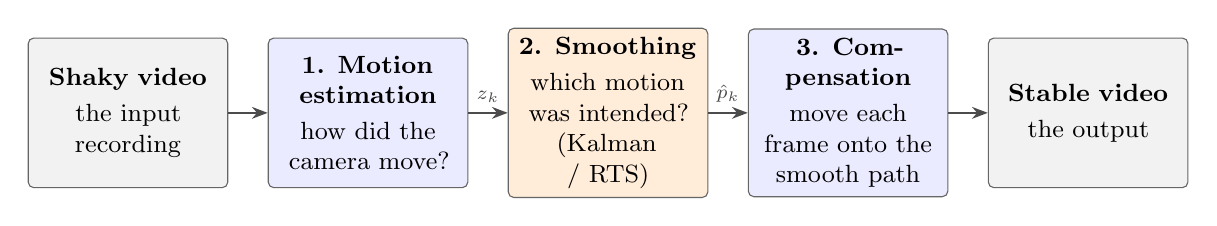
\begin{tikzpicture}[
      node distance=5mm,
      box/.style={draw=black!60, rounded corners=2pt, fill=#1, align=center,
                  text width=2.3cm, minimum height=1.9cm, font=\small},
      box/.default={black!5},
      arr/.style={-{Stealth[length=2mm]}, thick, black!70}]
    \node[box] (in) {\textbf{Shaky video}\\[2pt] the input recording};
    \node[box={blue!8}, right=of in] (me) {\textbf{1. Motion estimation}\\[2pt]
          how did the camera move?};
    \node[box={orange!15}, right=of me] (sm) {\textbf{2. Smoothing}\\[2pt]
          which motion was intended? (Kalman / RTS)};
    \node[box={blue!8}, right=of sm] (mc) {\textbf{3. Compensation}\\[2pt]
          move each frame onto the smooth path};
    \node[box, right=of mc] (out) {\textbf{Stable video}\\[2pt] the output};
    \draw[arr] (in) -- (me);
    \draw[arr] (me) -- node[above, font=\scriptsize] {$z_k$} (sm);
    \draw[arr] (sm) -- node[above, font=\scriptsize] {$\hat p_k$} (mc);
    \draw[arr] (mc) -- (out);
  \end{tikzpicture}
  \caption{The three stages of digital stabilisation. $z_k$ is the raw (shaky) camera path
  measured at frame $k$, and $\hat p_k$ is the estimated intended path.}
  \label{fig:pipeline}
\end{figure}

\subsection{The Kalman filter in brief}
A Kalman filter estimates a quantity that cannot be observed directly, using noisy
measurements of it and a model of how it behaves. Here the hidden quantity is the camera's
intended path and the measurement is the shaky raw path. The filter repeats two steps for
every frame:
\begin{itemize}
  \item \textbf{Predict.} Use the motion model to guess where the intended path will be in
        this frame. For example, if the camera was panning at 2\,px per frame, it will
        probably move another 2\,px.
  \item \textbf{Update.} Compare the guess with the measured position, and move the guess
        part of the way towards the measurement.
\end{itemize}
How far the guess moves depends on how much each source is trusted. Two numbers control
this. $R$ is the size of the shake: a large $R$ means the measurements are unreliable, so the
filter trusts its prediction more and the output is smoother. $Q$ is how quickly the intended
motion may change: a large $Q$ means the camera can start and stop turning quickly, so the
filter follows the measurements more closely. In this report a single ratio $\rho = Q/R$ sets
the balance.

As well as an estimate, the filter keeps track of how uncertain it is. This makes it possible
to check whether the filter's assumptions hold (Section~\ref{sec:consistency}).

\subsection{Filtering versus smoothing}
The Kalman filter only uses frames up to the current one. This means it is \emph{causal} and
can run on a live video. The drawback is lag: when the camera starts a deliberate pan, the
filter needs a few frames to notice, so it falls behind.

A recorded video can also be processed \emph{offline}, using future frames. The
Rauch--Tung--Striebel (RTS) smoother~\cite{rts1965} runs a second pass backwards in time over
the Kalman filter's results, so every estimate uses the whole recording. It removes the lag,
but it cannot be used live.

\subsection{Key terms}
Table~\ref{tab:terms} lists the terms and symbols used in the rest of the report.

\begin{table}[htbp]
  \centering
  \small
  \caption{Key terms and symbols.}
  \label{tab:terms}
  \begin{tabularx}{\linewidth}{@{}lX@{}}
    \toprule
    Term & Meaning \\
    \midrule
    Path (trajectory) & The camera's horizontal position $x$, vertical position $y$ and
                        rotation $\theta$, one value per frame. \\
    Intended path $p_k$ & The smooth motion the person filming wanted, such as a steady pan.
                          It is unknown and is what we estimate. \\
    Shake & Small, fast, unwanted motion on top of the intended path. \\
    Raw path $z_k$ & The camera path measured from the video: intended motion plus shake. \\
    Estimate $\hat p_k$ & Our best estimate of the intended path at frame $k$. \\
    State $\mathbf{x}_k$ & What the filter tracks: the position $p_k$ and velocity $v_k$ of
                           the intended path. \\
    Process noise $Q$ & How much the intended motion may change speed from one frame to the
                        next. \\
    Measurement noise $R$ & How far the raw path wanders from the intended path; the size of
                            the shake. \\
    Ratio $\rho = Q/R$ & The single tuning parameter. A smaller $\rho$ gives a smoother output
                         that is slower to follow real turns. \\
    Kalman gain $K_k$ & How strongly each new measurement corrects the prediction. \\
    Innovation $\nu_k$ & The ``surprise'': measured position minus predicted position. \\
    Causal / offline & Uses only past frames (can run live) / uses the whole recording. \\
    \bottomrule
  \end{tabularx}
\end{table}

\subsection{Related work}
Kalman filters have been used for video stabilisation for many years~\cite{litvin2003}. Other
approaches smooth the path with a Gaussian filter~\cite{matsushita2006}, or choose an optimal
camera path made of constant, linear and parabolic segments~\cite{grundmann2011}. An
open-source student project applies a simpler random-walk Kalman filter to each motion
parameter~\cite{spoorthiuk}. This report uses a constant-velocity model instead, adds the RTS
smoother, and measures the results against a known ground truth.

% =====================================================================
\section{Method}\label{sec:method}
% =====================================================================

\subsection{Measuring the camera's motion}\label{sec:motion}
To find how the camera moved between two frames, we pick points that are easy to follow, see
where they went, and fit one motion that explains most of them.
\begin{enumerate}
  \item \textbf{Find corners.} Up to 400 Shi--Tomasi corners~\cite{shitomasi1994} are
        detected in frame $k-1$ (quality level $0.01$, at least 15\,px apart). Corners can
        be located precisely, unlike points on a plain wall or along a straight edge.
  \item \textbf{Track them.} Pyramidal Lucas--Kanade optical
        flow~\cite{lucaskanade1981,bouguet2001} finds where each corner moved to in frame $k$.
  \item \textbf{Fit one motion.} A similarity transform (a rotation $\Delta\theta_k$ and a
        translation $(\Delta x_k, \Delta y_k)$, plus a uniform scale that is not used) is
        fitted to the tracked points with RANSAC~\cite{fischler1981}, using a 3\,px
        threshold. RANSAC repeatedly fits the motion to small random sets of points and
        keeps the fit that most points agree with. Points that disagree, such as corners on
        a passing car or points that were tracked wrongly, are ignored.
\end{enumerate}
If tracking fails completely, the frame is assumed not to have moved. Adding up the
per-frame motion gives the raw camera path:
\begin{equation}
  z_k = \sum_{j=1}^{k} \bigl(\Delta x_j,\ \Delta y_j,\ \Delta\theta_j\bigr), \qquad z_0 = 0 .
\end{equation}
Figures~\ref{fig:tracking-synth} and~\ref{fig:tracking-real} show this step on two frame pairs
from each video.

\begin{figure}[htbp]
  \centering
  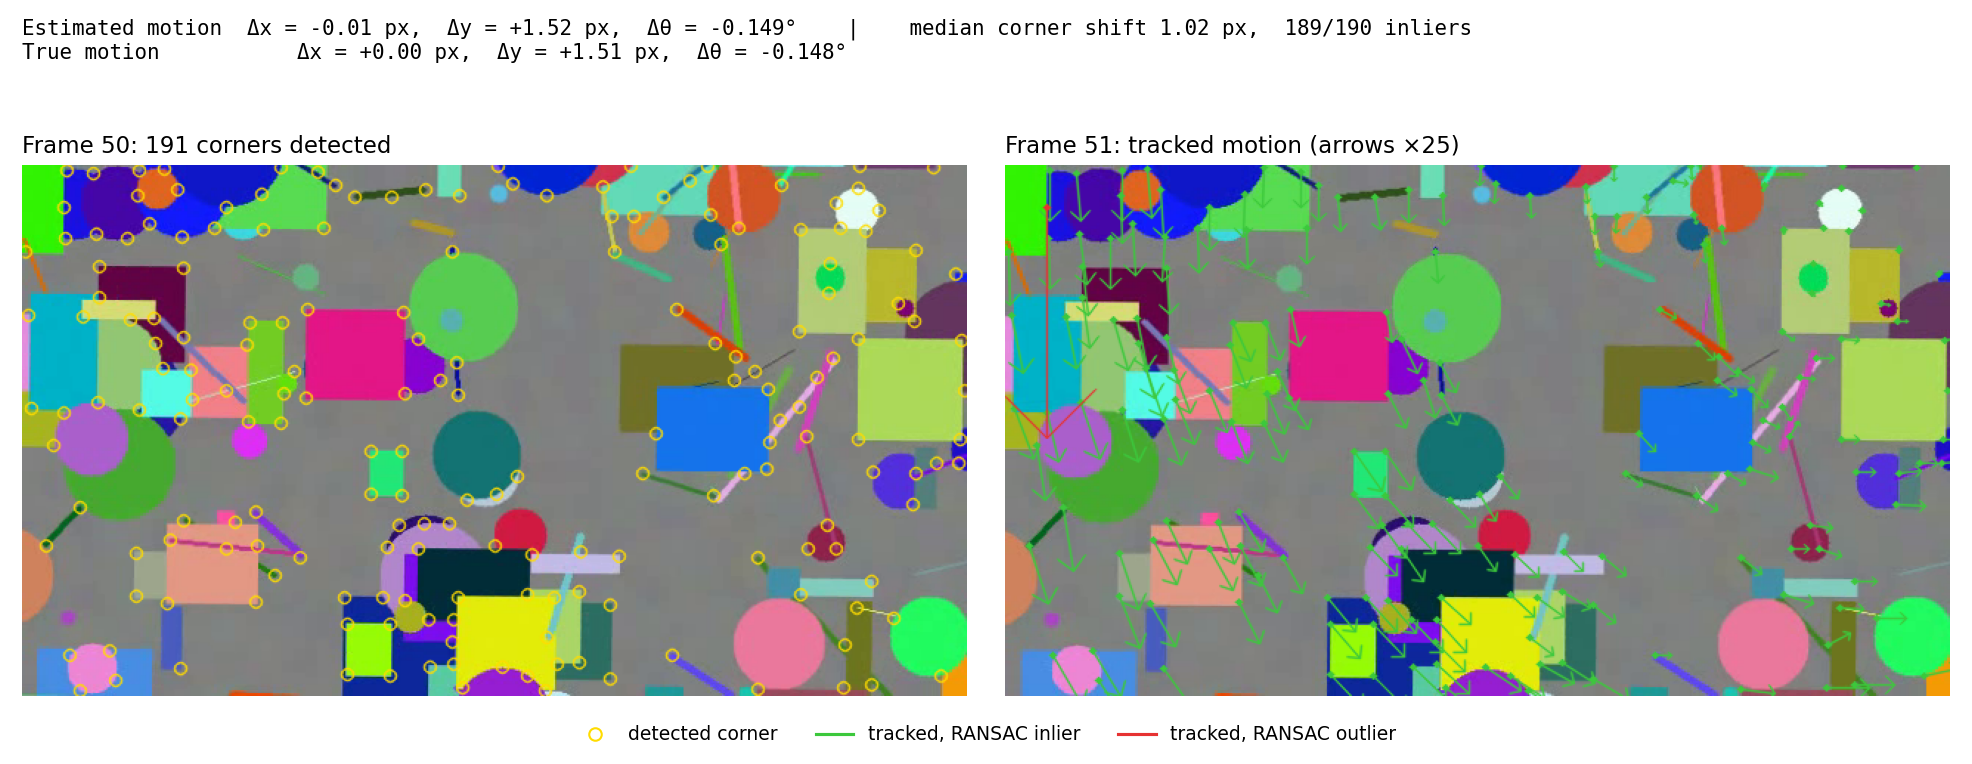
\includegraphics[width=\linewidth]{synth_tracking_50.png}\\[4pt]
  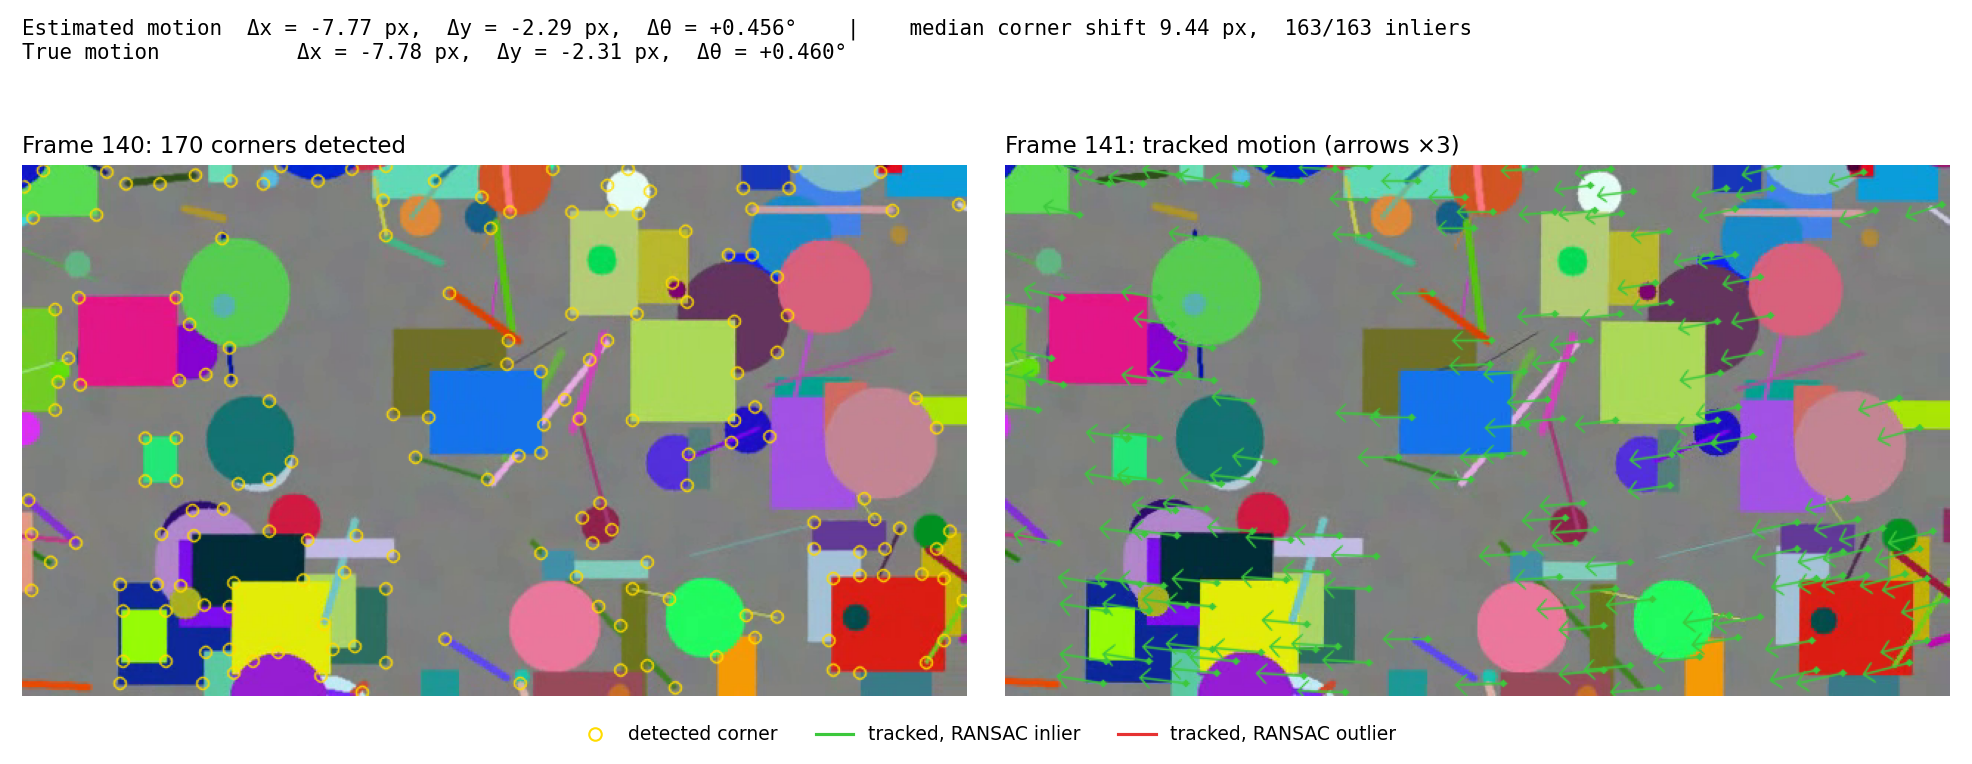
\includegraphics[width=\linewidth]{synth_tracking_140.png}
  \caption{Motion estimation on the synthetic video. Left: corners found in frame $k$.
  Right: how far each corner moved by frame $k+1$ (arrows lengthened by the factor in the
  title so they are visible). Green arrows agree with the fitted motion; red ones were
  rejected by RANSAC. Top: frames 50$\to$51 (shake only). Bottom: frames 140$\to$141 (during
  the fast pan). The true motion is printed for comparison.}
  \label{fig:tracking-synth}
\end{figure}

\begin{figure}[htbp]
  \centering
  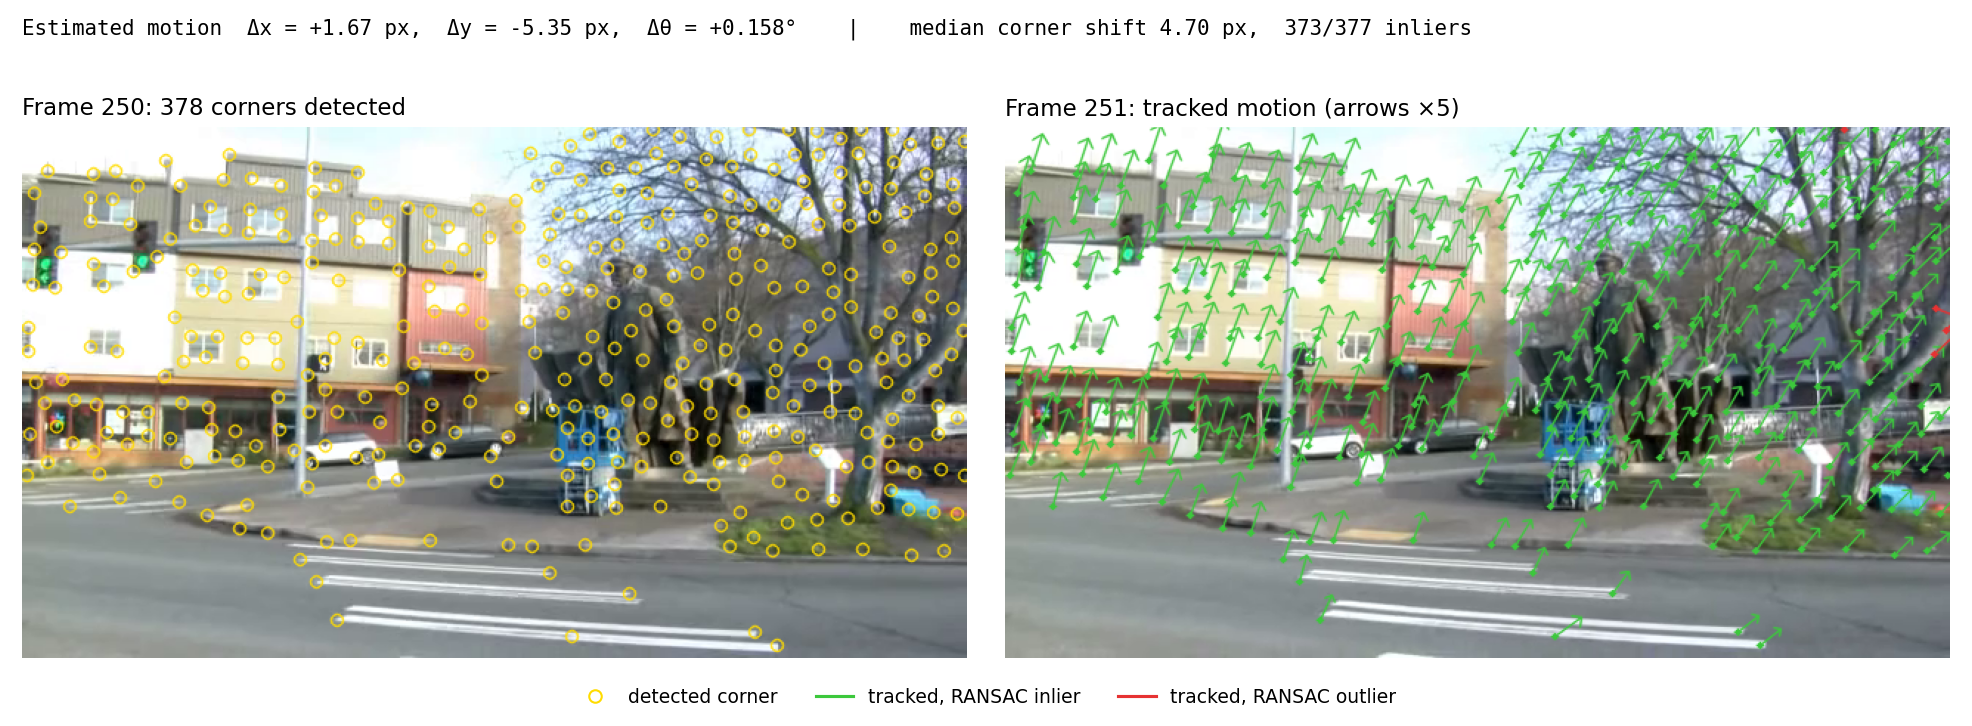
\includegraphics[width=\linewidth]{real_tracking_250.png}\\[4pt]
  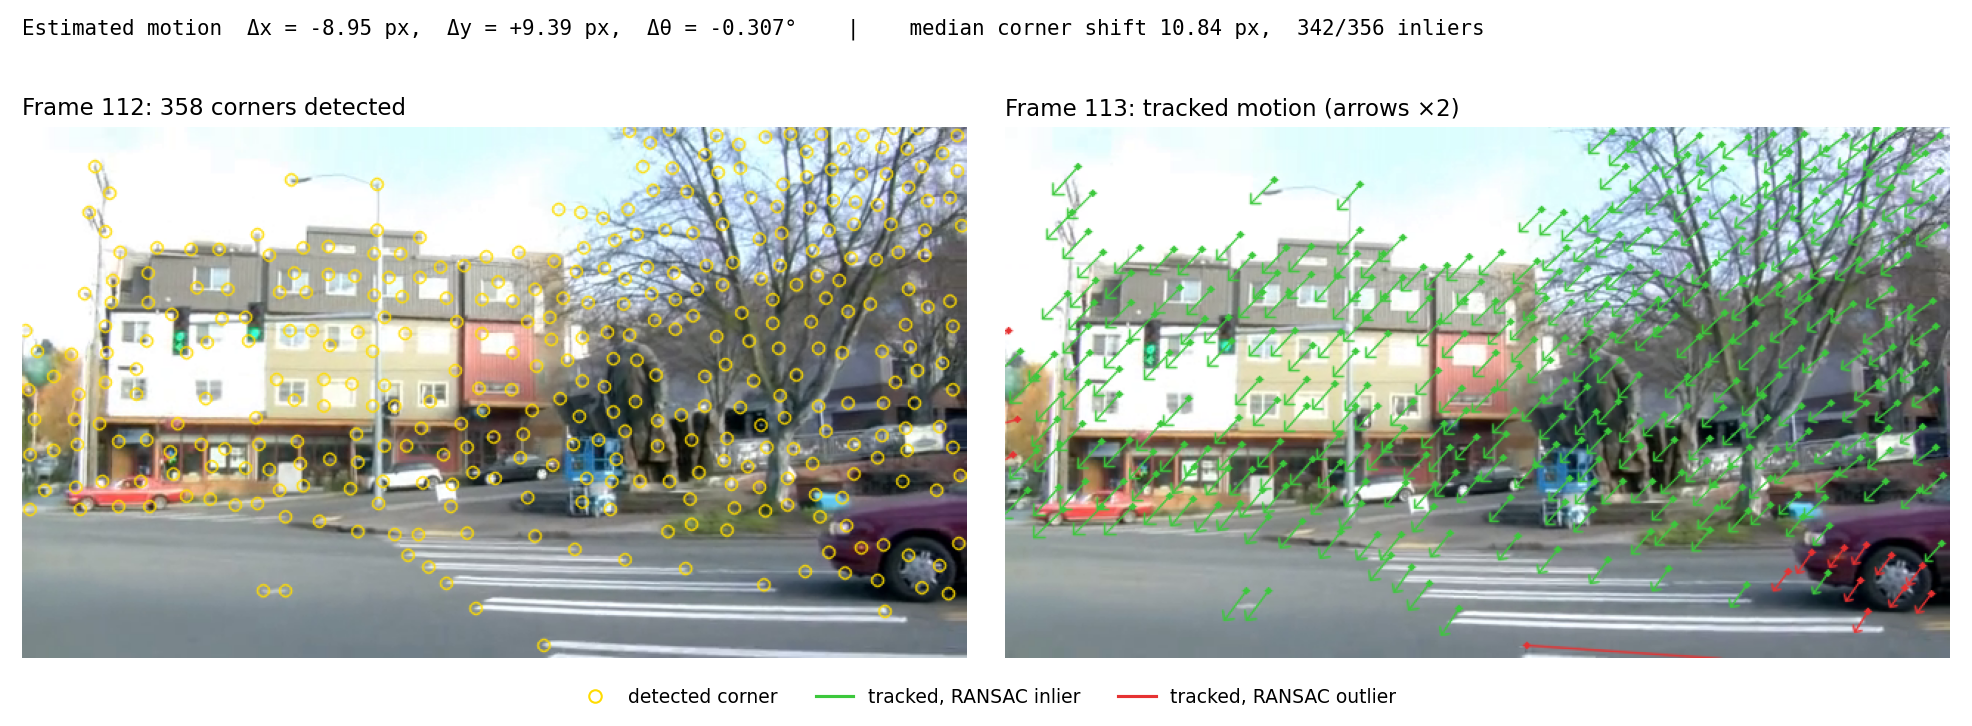
\includegraphics[width=\linewidth]{real_tracking_112.png}
  \caption{Motion estimation on the real video, drawn as in Figure~\ref{fig:tracking-synth}.
  Top: frames 250$\to$251. Bottom: frames 112$\to$113, the largest frame-to-frame motion in
  the clip. RANSAC rejects the corners on the moving car (red), because they do not move with
  the background.}
  \label{fig:tracking-real}
\end{figure}

\subsection{Motion model}\label{sec:model}
The filter needs a model of how the intended path behaves. We assume the camera moves at a
roughly constant speed that changes only gradually. The same model is used separately for
each of the three axes ($x$, $y$ and $\theta$), so three independent filters run side by side.
For one axis, the state is the position and velocity of the intended path,
$\mathbf{x}_k = [p_k,\ v_k]\T$, and the time step is one frame. This is the discrete
white-noise acceleration model~\cite{barshalom2001}:
\begin{align}
  \mathbf{x}_k &= F\,\mathbf{x}_{k-1} + \mathbf{w}_k, &
  F &= \begin{bmatrix} 1 & 1 \\ 0 & 1 \end{bmatrix}, &
  \mathbf{w}_k &\sim \mathcal{N}(0, Q), &
  Q &= q\,G G\T,\quad G = \begin{bmatrix} \tfrac12 \\ 1 \end{bmatrix}, \\
  z_k &= H\,\mathbf{x}_k + v_k, &
  H &= \begin{bmatrix} 1 & 0 \end{bmatrix}, &
  v_k &\sim \mathcal{N}(0, R). &&
\end{align}
In words:
\begin{itemize}
  \item $F$ says that the new position is the old position plus the velocity, and that the
        velocity stays the same.
  \item $\mathbf{w}_k$ lets the velocity change slightly each frame, as if pushed by a small
        random acceleration of variance $q$. $G$ converts that acceleration into a change of
        position ($\tfrac12$) and of velocity ($1$).
  \item $H$ says that only the position is measured, not the velocity.
  \item $v_k$ is the shake: the measured path is the intended path plus a random, zero-mean
        disturbance of variance $R$.
\end{itemize}

\subsection{Kalman filter}\label{sec:kf}
The filter starts from $\hat{\mathbf{x}}_{0|-1} = [z_0,\ 0]\T$ (first measured position, zero
velocity) with uncertainty $P_{0|-1} = \operatorname{diag}(R, R)$. The subscript $k|k-1$ means
``at frame $k$, using measurements up to frame $k-1$''. For every frame it then performs:
\begin{align}
  \text{predict:}\quad & \hat{\mathbf{x}}_{k|k-1} = F\,\hat{\mathbf{x}}_{k-1|k-1}, &
  P_{k|k-1} &= F P_{k-1|k-1} F\T + Q, \\
  \text{surprise:}\quad & \nu_k = z_k - H\hat{\mathbf{x}}_{k|k-1}, &
  S_k &= H P_{k|k-1} H\T + R, \\
  \text{gain:}\quad & K_k = P_{k|k-1} H\T S_k^{-1}, && \\
  \text{update:}\quad & \hat{\mathbf{x}}_{k|k} = \hat{\mathbf{x}}_{k|k-1} + K_k \nu_k, &
  P_{k|k} &= (I - K_k H) P_{k|k-1} (I - K_k H)\T + K_k R K_k\T .
\end{align}
$P$ is the filter's uncertainty about its state, and $S_k$ is the size of surprise it expects.
The gain $K_k$ is large when the prediction is uncertain compared with the measurement, and
small otherwise. The covariance update is written in the Joseph form, which keeps $P$
symmetric and positive definite despite rounding errors. The live estimate of the intended
path is the position part of the state, $\hat p_k = [\hat{\mathbf{x}}_{k|k}]_1$.

\subsection{RTS smoother}\label{sec:rts}
For a recorded video, the RTS smoother~\cite{rts1965} runs backwards over the stored filter
results, for $k = N-1, \dots, 0$:
\begin{align}
  C_k &= P_{k|k} F\T P_{k+1|k}^{-1}, \\
  \hat{\mathbf{x}}_{k|N} &= \hat{\mathbf{x}}_{k|k} + C_k \bigl(\hat{\mathbf{x}}_{k+1|N} - \hat{\mathbf{x}}_{k+1|k}\bigr), \\
  P_{k|N} &= P_{k|k} + C_k \bigl(P_{k+1|N} - P_{k+1|k}\bigr) C_k\T .
\end{align}
Each step corrects the forward estimate at frame $k$ by how much the (already smoothed) next
frame differs from what the filter had predicted for it. As a result every smoothed estimate
uses all $N$ frames, which removes the lag the live filter has on deliberate motion.

\subsection{Choosing the noise levels}\label{sec:noise}
The shake size $R$ is estimated from the video itself, separately for each axis. A centred
15-frame moving average ($\operatorname{MA}_{15}$) removes the fast shake and keeps the slow
motion, so what is left over is roughly the shake:
\begin{equation}
  R = \operatorname{Var}\bigl(z_k - \operatorname{MA}_{15}(z)_k\bigr).
\end{equation}
The process noise is then set relative to it, $q = \rho R$. This leaves a single tuning
parameter, $\rho = Q/R$, for all three axes (default $\rho = 3\times10^{-4}$). A smaller $\rho$
tells the filter to trust its motion model more. The output is then smoother, but lags more
behind real turns.

\subsection{Baselines}
To show what the Kalman approach adds, it is compared with two moving averages, each over 15
frames. The \emph{causal} moving average uses the current and 14 previous frames, so like the
Kalman filter it could run live. The \emph{centred} moving average uses 7 frames on either side,
so like the RTS smoother it needs the recording.

\subsection{Motion compensation}\label{sec:comp}
Each frame is moved by the correction $\Delta_k = \hat p_k - z_k$, the gap between where the
camera should have been and where it was. This is a rotation by $\Delta_k^\theta$ and a shift
by $(\Delta_k^x, \Delta_k^y)$. Moving a frame leaves black borders at its edges, so every frame
is also enlarged by $s = 1.12$ about its centre to push the borders out of view. At
$640\times360$ this hides corrections of up to $38.4$\,px horizontally and $21.6$\,px
vertically.

% =====================================================================
\section{Implementation}\label{sec:impl}
% =====================================================================
The pipeline is written in Python 3. NumPy is used for the filter, OpenCV for corner tracking
and image warping, and Matplotlib for the plots. The Kalman filter and RTS smoother are written
from scratch rather than taken from a library. The code is in three files:
\begin{itemize}
  \item \texttt{kalman.py}: the motion model, Kalman filter, RTS smoother and moving averages;
  \item \texttt{stabilize.py}: motion estimation, smoothing, compensation and evaluation;
  \item \texttt{synth\_video.py}: generates the synthetic test video and its ground truth.
\end{itemize}
The listings below are excerpts of the key routines. Lines that only create or store arrays
are replaced by \texttt{...}.

\subsection{Motion estimation}
Listing~\ref{lst:motion} handles one pair of consecutive frames
(Section~\ref{sec:motion}). The rotation angle is read from the fitted $2\times3$ matrix as
$\operatorname{atan2}(m_{21}, m_{11})$, which ignores the unused scale factor.

\begin{lstlisting}[caption={Measuring the motion between two frames (\texttt{stabilize.py}).},label=lst:motion]
pts = cv2.goodFeaturesToTrack(prev_gray, maxCorners=400, qualityLevel=0.01,
                              minDistance=15, blockSize=3)       # Shi-Tomasi corners
m = None
if pts is not None and len(pts) >= 10:
    nxt, st, _ = cv2.calcOpticalFlowPyrLK(prev_gray, gray, pts, None)  # pyramidal LK
    good = st.ravel() == 1
    if good.sum() >= 10:
        m, inl = cv2.estimateAffinePartial2D(pts[good], nxt[good],   # similarity + RANSAC
                                             method=cv2.RANSAC,
                                             ransacReprojThreshold=3.0)
if m is None:                      # tracking failed: assume no motion
    transforms.append((0.0, 0.0, 0.0))
else:
    transforms.append((m[0, 2], m[1, 2], np.arctan2(m[1, 0], m[0, 0])))
...
raw = np.vstack([np.zeros(3), np.cumsum(transforms, axis=0)])   # raw path z_k
\end{lstlisting}

\subsection{Motion model and Kalman filter}
Listing~\ref{lst:model} builds the matrices of Section~\ref{sec:model}, and
Listing~\ref{lst:kf} is the filter loop of Section~\ref{sec:kf}. Because only one number is
measured per frame, $S_k$ is a single number and the gain is a division rather than a matrix
inverse. The predicted and updated states and uncertainties are stored for every frame,
because the RTS smoother needs them. The surprises $\nu_k$ and their expected sizes $S_k$ are
stored for the consistency tests.

\begin{lstlisting}[caption={Constant-velocity motion model (\texttt{kalman.py}).},label=lst:model]
def cv_model(q, r, dt=1.0):
    """Return F, H, Q, R for the constant-velocity model."""
    F = np.array([[1.0, dt],
                  [0.0, 1.0]])
    H = np.array([[1.0, 0.0]])
    G = np.array([[0.5 * dt ** 2],
                  [dt]])
    Q = q * (G @ G.T)           # discrete white-noise acceleration
    R = np.array([[r]])
    return F, H, Q, R
\end{lstlisting}

\begin{lstlisting}[caption={Kalman filter predict and update loop (\texttt{kalman.py}).},label=lst:kf]
def kalman_filter(z, F, H, Q, R, x0=None, P0=None):
    n, nx = len(z), F.shape[0]
    I = np.eye(nx)
    if x0 is None:
        x0 = np.array([z[0], 0.0])          # start at first measurement, zero velocity
    if P0 is None:
        P0 = np.diag([R[0, 0], R[0, 0]])
    ...                                     # allocate x_pred, P_pred, x_filt, P_filt, ...
    for k in range(n):
        # ---- Predict ----
        if k == 0:
            xp, Pp = x0, P0
        else:
            xp = F @ x_filt[k - 1]
            Pp = F @ P_filt[k - 1] @ F.T + Q
        # ---- Update ----
        y = z[k] - (H @ xp)[0]              # innovation
        S = (H @ Pp @ H.T + R)[0, 0]        # innovation covariance
        K = (Pp @ H.T)[:, 0] / S            # Kalman gain
        xf = xp + K * y
        KH = np.outer(K, H[0])
        # Joseph form: keeps P symmetric positive definite
        Pf = (I - KH) @ Pp @ (I - KH).T + np.outer(K, K) * R[0, 0]
        ...                                 # store xp, Pp, xf, Pf, K, y, S for frame k
\end{lstlisting}

\subsection{RTS smoother}
Listing~\ref{lst:rts} is the backward pass of Section~\ref{sec:rts}. It starts from the last
frame, where the filter's estimate is already the smoothed one, and works back to the first.

\begin{lstlisting}[caption={Rauch--Tung--Striebel backward pass (\texttt{kalman.py}).},label=lst:rts]
def rts_smoother(kf, F):
    x_f, P_f = kf["x_filt"], kf["P_filt"]
    x_p, P_p = kf["x_pred"], kf["P_pred"]
    n = len(x_f)
    x_s, P_s = x_f.copy(), P_f.copy()
    for k in range(n - 2, -1, -1):
        C = P_f[k] @ F.T @ np.linalg.inv(P_p[k + 1])     # smoother gain
        x_s[k] = x_f[k] + C @ (x_s[k + 1] - x_p[k + 1])
        P_s[k] = P_f[k] + C @ (P_s[k + 1] - P_p[k + 1]) @ C.T
    return {"x_smooth": x_s, "P_smooth": P_s}
\end{lstlisting}

\subsection{Noise levels and smoothing each axis}
Listing~\ref{lst:smooth} estimates $R$ from the video (Section~\ref{sec:noise}) and runs the
filter and smoother on each axis with $q = \rho R$. The moving-average baselines are computed
in the same loop.

\begin{lstlisting}[caption={Estimating $R$ and smoothing each axis (\texttt{stabilize.py}).},label=lst:smooth]
def estimate_R(traj, window=15):
    R = []
    for a in range(traj.shape[1]):
        resid = traj[:, a] - moving_average(traj[:, a], window)  # high-frequency residual
        R.append(max(np.var(resid), 1e-10))
    return np.array(R)

def smooth(traj, q_ratio, R, ma_window):
    ...
    for a, name in enumerate(AXES):                     # x, y, theta independently
        z = traj[:, a]
        F, H, Q, Rm = cv_model(q=q_ratio * R[a], r=R[a])
        kf = kalman_filter(z, F, H, Q, Rm)
        rts = rts_smoother(kf, F)
        out["kf"][:, a] = kf["x_filt"][:, 0]            # live estimate of p_k
        out["rts"][:, a] = rts["x_smooth"][:, 0]        # offline estimate of p_k
        out["ma_causal"][:, a] = moving_average(z, ma_window, causal=True)
        out["ma_centred"][:, a] = moving_average(z, ma_window, causal=False)
\end{lstlisting}

\subsection{Motion compensation}
Listing~\ref{lst:warp} builds the warp for frame $k$ from the correction
$\Delta_k = \hat p_k - z_k$ (Section~\ref{sec:comp}). The rotation and shift are applied first,
then the enlargement about the image centre.

\begin{lstlisting}[caption={Correction warp and border zoom (\texttt{stabilize.py}).},label=lst:warp]
def correction_matrix(corr, zoom, w, h):
    dx, dy, da = corr
    c, s = np.cos(da), np.sin(da)
    M = np.array([[c, -s, dx], [s, c, dy], [0, 0, 1.0]])       # rotate + translate
    Z = np.array([[zoom, 0, (1 - zoom) * w / 2],               # zoom about the centre
                  [0, zoom, (1 - zoom) * h / 2],
                  [0, 0, 1.0]])
    return (Z @ M)[:2]

corrections = paths[method] - raw_traj                         # Delta_k for every frame
M = correction_matrix(corrections[k], zoom, w, h)
stabilised = cv2.warpAffine(frame, M, (w, h), borderMode=cv2.BORDER_CONSTANT)
\end{lstlisting}

% =====================================================================
\section{Experimental setup}\label{sec:setup}
% =====================================================================

\subsection{Synthetic video}
With a real video we never know the true intended path, so we cannot measure how close a
method gets to it. A synthetic video solves this. A virtual $640\times360$ camera films a large
scene filled with 450 random rectangles, circles and lines, which gives plenty of corners to
track. The camera's intended path is:
\begin{itemize}
  \item a slow horizontal pan at 1\,px per frame;
  \item a deliberate fast pan between 40\% and 55\% of the clip (frames 120--165), where the
        speed rises smoothly by up to 7\,px per frame and falls back again (a raised-cosine
        profile);
  \item a gentle vertical drift of $15\sin t$\,px for $t \in [0, 1.5\pi]$.
\end{itemize}
Shake is added to $x$, $y$ and $\theta$ as random noise smoothed over a few frames (a Gaussian
kernel with $\sigma = 2$ frames), so that it looks like hand tremor, with a standard deviation
of 6\,px and $0.6^\circ$. Mild sensor noise ($\sigma = 2$ grey levels) is added to each frame.
The clip has 300 frames at 30\,fps, and the true shaky and intended camera positions are saved
for every frame.

\subsection{Real video}
The real video is a hand-held recording of a street scene: $640\times360$ pixels, 495 frames
at 28.8\,fps (17.2\,s). The camera pans steadily, moving the view by about 550\,px horizontally
and 120\,px vertically over the clip, with the irregular shake typical of walking. There is no
ground truth for this video.
% TODO: state where the real video comes from (own recording or a public test clip).

\subsection{How the methods are scored}
Table~\ref{tab:metrics} summarises the metrics.

\begin{table}[htbp]
  \centering
  \small
  \caption{Evaluation metrics.}
  \label{tab:metrics}
  \begin{tabularx}{\linewidth}{@{}lXc@{}}
    \toprule
    Metric & What it measures & Better \\
    \midrule
    ITF (dB) & How similar each output frame is to the previous one. A steady video changes
               little between frames. & higher \\
    Jitter (px/frame$^2$) & How abruptly the path changes speed. A smooth path has low
                            jitter. & lower \\
    Max correction (px) & The largest shift applied to any frame. Larger shifts need more
                          cropping. & lower \\
    RMSE (px) & How far the estimated path is from the true intended path (synthetic video
                only). & lower \\
    NIS & Whether the filter's surprises are as large as it expects (filter consistency). &
          close to 1 \\
    \bottomrule
  \end{tabularx}
\end{table}

In detail:
\begin{itemize}
  \item \textbf{Inter-frame transformation fidelity (ITF)}~\cite{morimoto1998} is the mean
        PSNR (peak signal-to-noise ratio) between consecutive output frames. It is computed
        on the central 80\% of each greyscale frame to leave out the borders.
  \item \textbf{Jitter} is the root-mean-square second difference of the $x, y$ path,
        $J = \bigl(\frac{1}{2(N-2)} \sum_k \lVert \hat p_{k+1} - 2\hat p_k + \hat p_{k-1}\rVert^2\bigr)^{1/2}$.
  \item \textbf{Maximum correction} is the largest $|\Delta_k^x|$ or $|\Delta_k^y|$ over the
        clip.
  \item \textbf{RMSE to the intended path} is the root-mean-square distance between the
        estimated and true $x, y$ paths, after removing the best constant offset. The offset
        is removed because frame 0 already contains shake, so the absolute position of the
        output is arbitrary; only the shape of the path matters.
  \item \textbf{Filter consistency} uses the normalised innovation squared (NIS),
        $\epsilon_k = \nu_k^2 / S_k$: the actual surprise divided by the surprise the filter
        expected. If the filter's assumptions are right, its average is 1 and about 95\% of
        innovations fall inside $\pm 2\sqrt{S_k}$~\cite{barshalom2001}.
\end{itemize}

\subsection{Settings}
Table~\ref{tab:settings} lists the settings. They are the same for both videos.

\begin{table}[htbp]
  \centering
  \caption{Settings and estimated measurement noise.}
  \label{tab:settings}
  \begin{tabular}{lcc}
    \toprule
    Parameter & Synthetic & Real \\
    \midrule
    Frames / frame rate & 300 / 30.0\,fps & 495 / 28.8\,fps \\
    Resolution & $640\times360$ & $640\times360$ \\
    Noise ratio $\rho = Q/R$ & $3\times10^{-4}$ & $3\times10^{-4}$ \\
    Moving-average window & 15 frames & 15 frames \\
    Border zoom $s$ & 1.12 & 1.12 \\
    Estimated $R_x$ / $R_y$ (px$^2$) & 20.69 / 17.84 & 20.23 / 34.55 \\
    Estimated $R_\theta$ (rad$^2$) & $7.08\times10^{-5}$ & $2.34\times10^{-5}$ \\
    Mean RANSAC inlier ratio & 0.996 & 0.992 \\
    \bottomrule
  \end{tabular}
\end{table}

% =====================================================================
\section{Results: synthetic video}\label{sec:res-synth}
% =====================================================================

\begin{keybox}
\textbf{In short.} The camera motion is measured accurately (0.89\,px error). The RTS smoother
is the best method overall: it gets closest to the true intended path and has about a third of
the jitter of the best baseline. Among the live methods, the Kalman filter follows the fast pan
far better than the causal moving average, but lets more shake through.
\end{keybox}

\subsection{Motion estimation}
The measured raw path matches the true shaky path with an RMSE of $0.89$\,px over the 300
frames. For the frame pairs in Figure~\ref{fig:tracking-synth}, the measured motion is within
$0.02$\,px and $0.004^\circ$ of the truth, both for pure shake (frame 50) and during the fast pan
(frame 140). Motion estimation is therefore accurate, and the differences between the methods
below come from the smoothing stage.

\subsection{Stabilisation}
Table~\ref{tab:synth} gives the scores and Figure~\ref{fig:synth-traj} the paths.

\begin{table}[htbp]
  \centering
  \caption{Results on the synthetic video. Arrows show whether higher or lower is better; the
  best value in each column is in bold.}
  \label{tab:synth}
  \begin{tabular}{lcccc}
    \toprule
    Method & ITF (dB) $\uparrow$ & Jitter $\downarrow$ & Max corr.\ (px) $\downarrow$ & RMSE (px) $\downarrow$ \\
    \midrule
    Raw (shaky)              & 25.82 & 1.314 & 0.0  & 8.68 \\
    Moving average, causal   & 31.36 & 0.211 & 56.5 & 10.82 \\
    Kalman filter (causal)   & 30.34 & 0.423 & 22.0 & 7.80 \\
    Moving average, centred  & 31.19 & 0.212 & \textbf{15.3} & 5.79 \\
    RTS smoother (offline)   & \textbf{31.74} & \textbf{0.063} & 17.3 & \textbf{5.75} \\
    \bottomrule
  \end{tabular}
\end{table}

\begin{figure}[htbp]
  \centering
  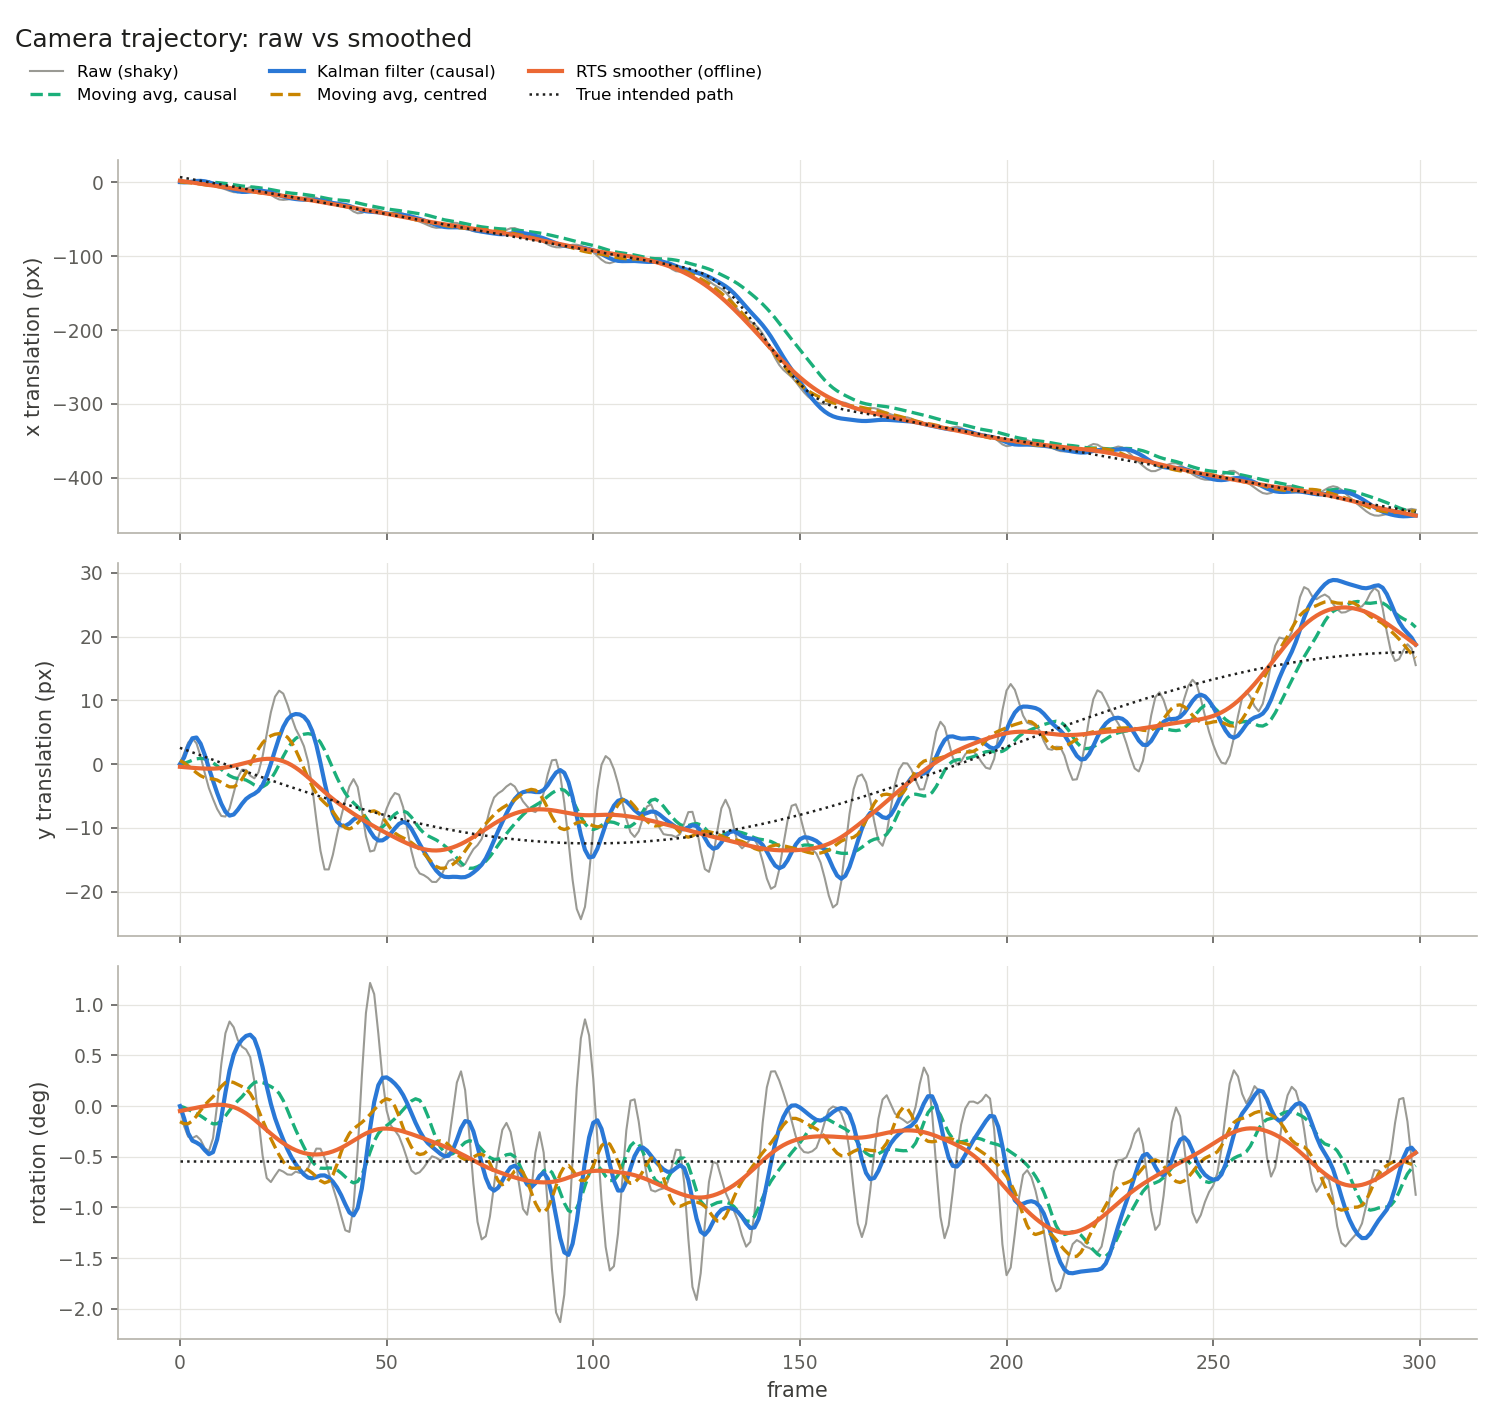
\includegraphics[width=0.85\linewidth]{synth_trajectories.png}
  \caption{Camera path on the synthetic video for $x$, $y$ and rotation: the raw (shaky) path,
  the four smoothing methods, and the true intended path.}
  \label{fig:synth-traj}
\end{figure}

\paragraph{The offline methods.} The RTS smoother is best on three of the four metrics. Its
jitter ($0.063$) is about 30\% of that of the centred moving average ($0.212$), the best
baseline, and its error to the intended path is the lowest of all. The constant-velocity model
describes a slowly changing pan better than a plain average does, so the RTS smoother can remove
more shake without bending the intended motion.

\paragraph{The live methods.} Here there is a clear trade-off. The causal moving average is
smoother than the Kalman filter (jitter $0.211$ against $0.423$), but it lags behind: a
15-frame trailing average is effectively 7 frames late. During the fast pan it falls far
behind, needs corrections of up to $56.5$\,px, and its RMSE ($10.82$\,px) is even worse than
the unstabilised video. The Kalman filter follows the pan more closely (maximum correction
$22.0$\,px, RMSE $7.80$\,px), but lets more shake through. Figure~\ref{fig:synth-pan} shows the
pan up close: both live methods lag at the start, and the Kalman filter overshoots at the end
because its velocity estimate takes time to slow down. Both offline methods stay close to the
true path throughout.

\begin{figure}[htbp]
  \centering
  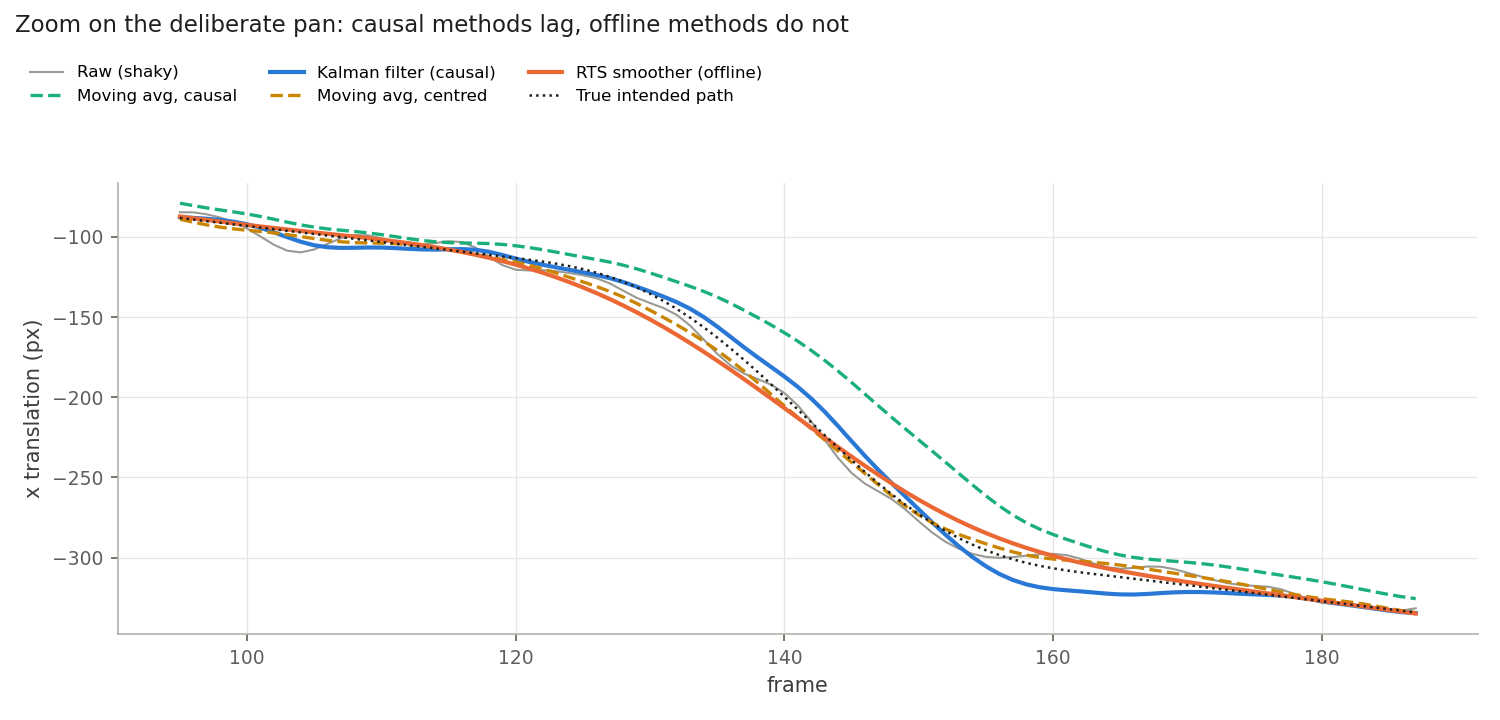
\includegraphics[width=0.95\linewidth]{synth_trajectories_pan_zoom.png}
  \caption{Close-up of the horizontal path around the fast pan (synthetic video).}
  \label{fig:synth-pan}
\end{figure}

\paragraph{Changing the tuning.} Figure~\ref{fig:synth-tradeoff} repeats the experiment for
many settings: $\rho$ from $10^{-6}$ to $1$ for the Kalman filter and RTS smoother, and windows
from 3 to 91 frames for the moving averages. Each curve shows how faithful a method can be for
a given smoothness. The RTS curve lies below all the others, so for any level of smoothness it
is the most faithful to the intended path, reaching a minimum RMSE of about $5.4$\,px. At
moderate smoothing (jitter around $0.4$) the two live methods perform alike. At stronger
smoothing the Kalman filter's error grows faster than the causal moving average's, because a
very small $Q$ makes the filter hold on to the pan's speed for too long and overshoot.

\begin{figure}[htbp]
  \centering
  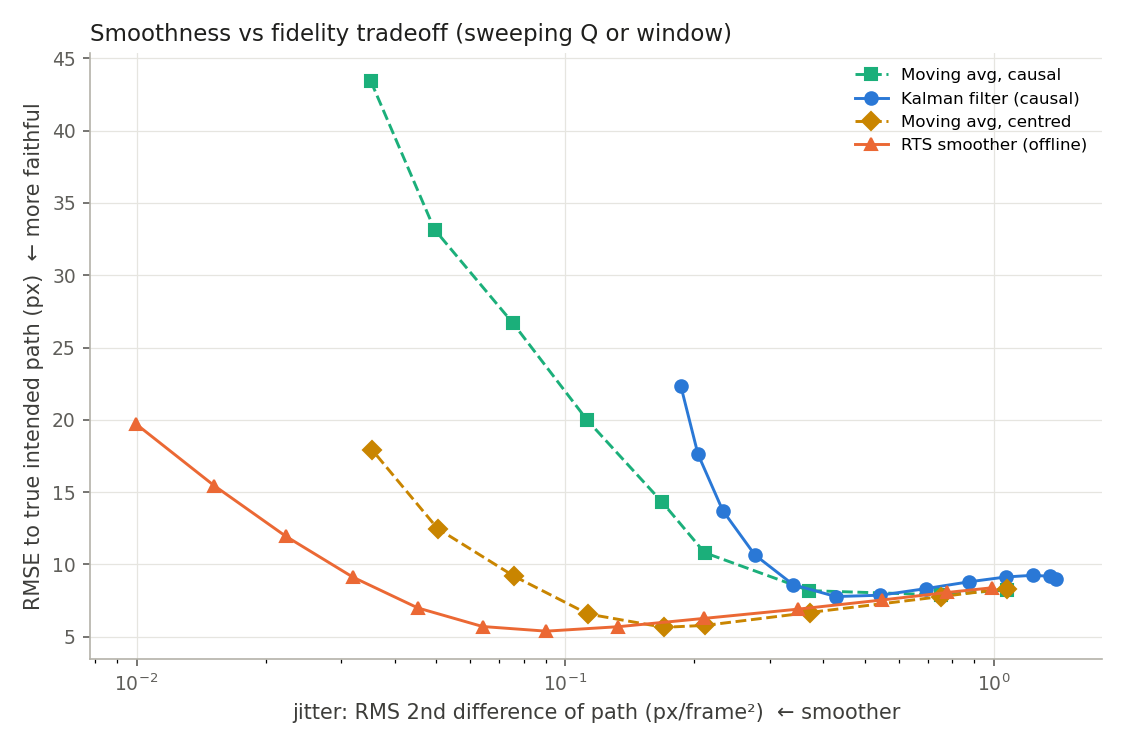
\includegraphics[width=0.7\linewidth]{synth_tradeoff_q_sweep.png}
  \caption{Smoothness against accuracy on the synthetic video, for a range of settings of
  $\rho = Q/R$ (Kalman filter, RTS) or the window length (moving averages). Down and to the
  left is better.}
  \label{fig:synth-tradeoff}
\end{figure}

\paragraph{What it looks like.} Figure~\ref{fig:synth-mean} averages ten consecutive output
frames. In a steady video the frames line up and the average stays sharp; any remaining shake
turns into blur. The raw video is strongly blurred and the Kalman filter output less so. The RTS
output is sharp apart from a horizontal smear of about 10\,px, which comes from the intended
1\,px-per-frame pan and should be kept.

\begin{figure}[htbp]
  \centering
  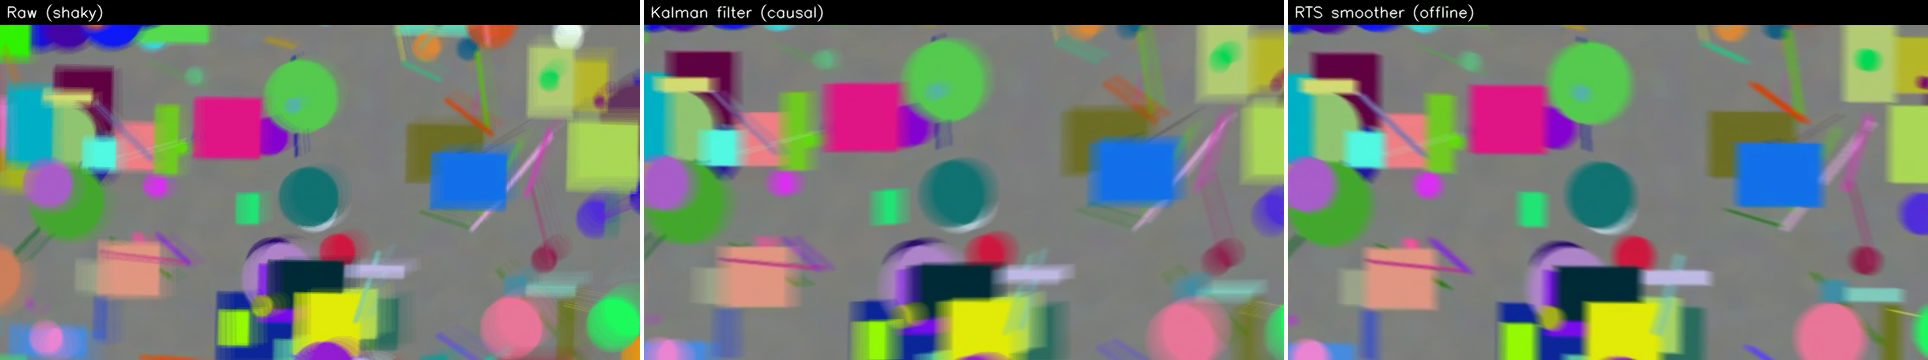
\includegraphics[width=\linewidth]{synth_temporal_mean.png}
  \caption{Average of 10 consecutive output frames (frames 40--49) of the synthetic video: raw,
  Kalman filter and RTS smoother. Remaining shake shows up as blur.}
  \label{fig:synth-mean}
\end{figure}

% =====================================================================
\section{Results: real video}\label{sec:res-real}
% =====================================================================

\begin{keybox}
\textbf{In short.} The results agree with the synthetic video. The RTS smoother gives the
steadiest output: frame-to-frame similarity rises from $18.7$ to $27.1$\,dB, and the jitter
is a quarter of either moving average's. Among the live methods, the Kalman filter needs less
correction than the causal moving average for the same smoothness.
\end{keybox}

Table~\ref{tab:real} gives the scores. With no ground truth there is no RMSE column, and the
trade-off plot uses the maximum correction instead.

\begin{table}[htbp]
  \centering
  \caption{Results on the real video. The best value in each column is in bold.}
  \label{tab:real}
  \begin{tabular}{lccc}
    \toprule
    Method & ITF (dB) $\uparrow$ & Jitter $\downarrow$ & Max corr.\ (px) $\downarrow$ \\
    \midrule
    Raw (shaky)              & 18.69 & 1.793 & 0.0 \\
    Moving average, causal   & 24.11 & 0.286 & 41.8 \\
    Kalman filter (causal)   & 21.92 & 0.524 & 26.5 \\
    Moving average, centred  & 24.18 & 0.286 & \textbf{20.5} \\
    RTS smoother (offline)   & \textbf{27.11} & \textbf{0.072} & 23.8 \\
    \bottomrule
  \end{tabular}
\end{table}

The RTS smoother raises the ITF by $8.4$\,dB over the raw video and by $2.9$\,dB over the best
baseline, and its jitter ($0.072$) is a quarter of that of either moving average. The live
trade-off is also the same as before: the causal moving average is smoother than the Kalman
filter but needs far more correction ($41.8$ against $26.5$\,px). Figure~\ref{fig:real-traj}
shows the paths. The shake is larger on this video, and largest in $y$
($R_y = 34.6$\,px$^2$ against $R_x = 20.2$\,px$^2$), which fits the up-and-down bounce of walking.

\begin{figure}[htbp]
  \centering
  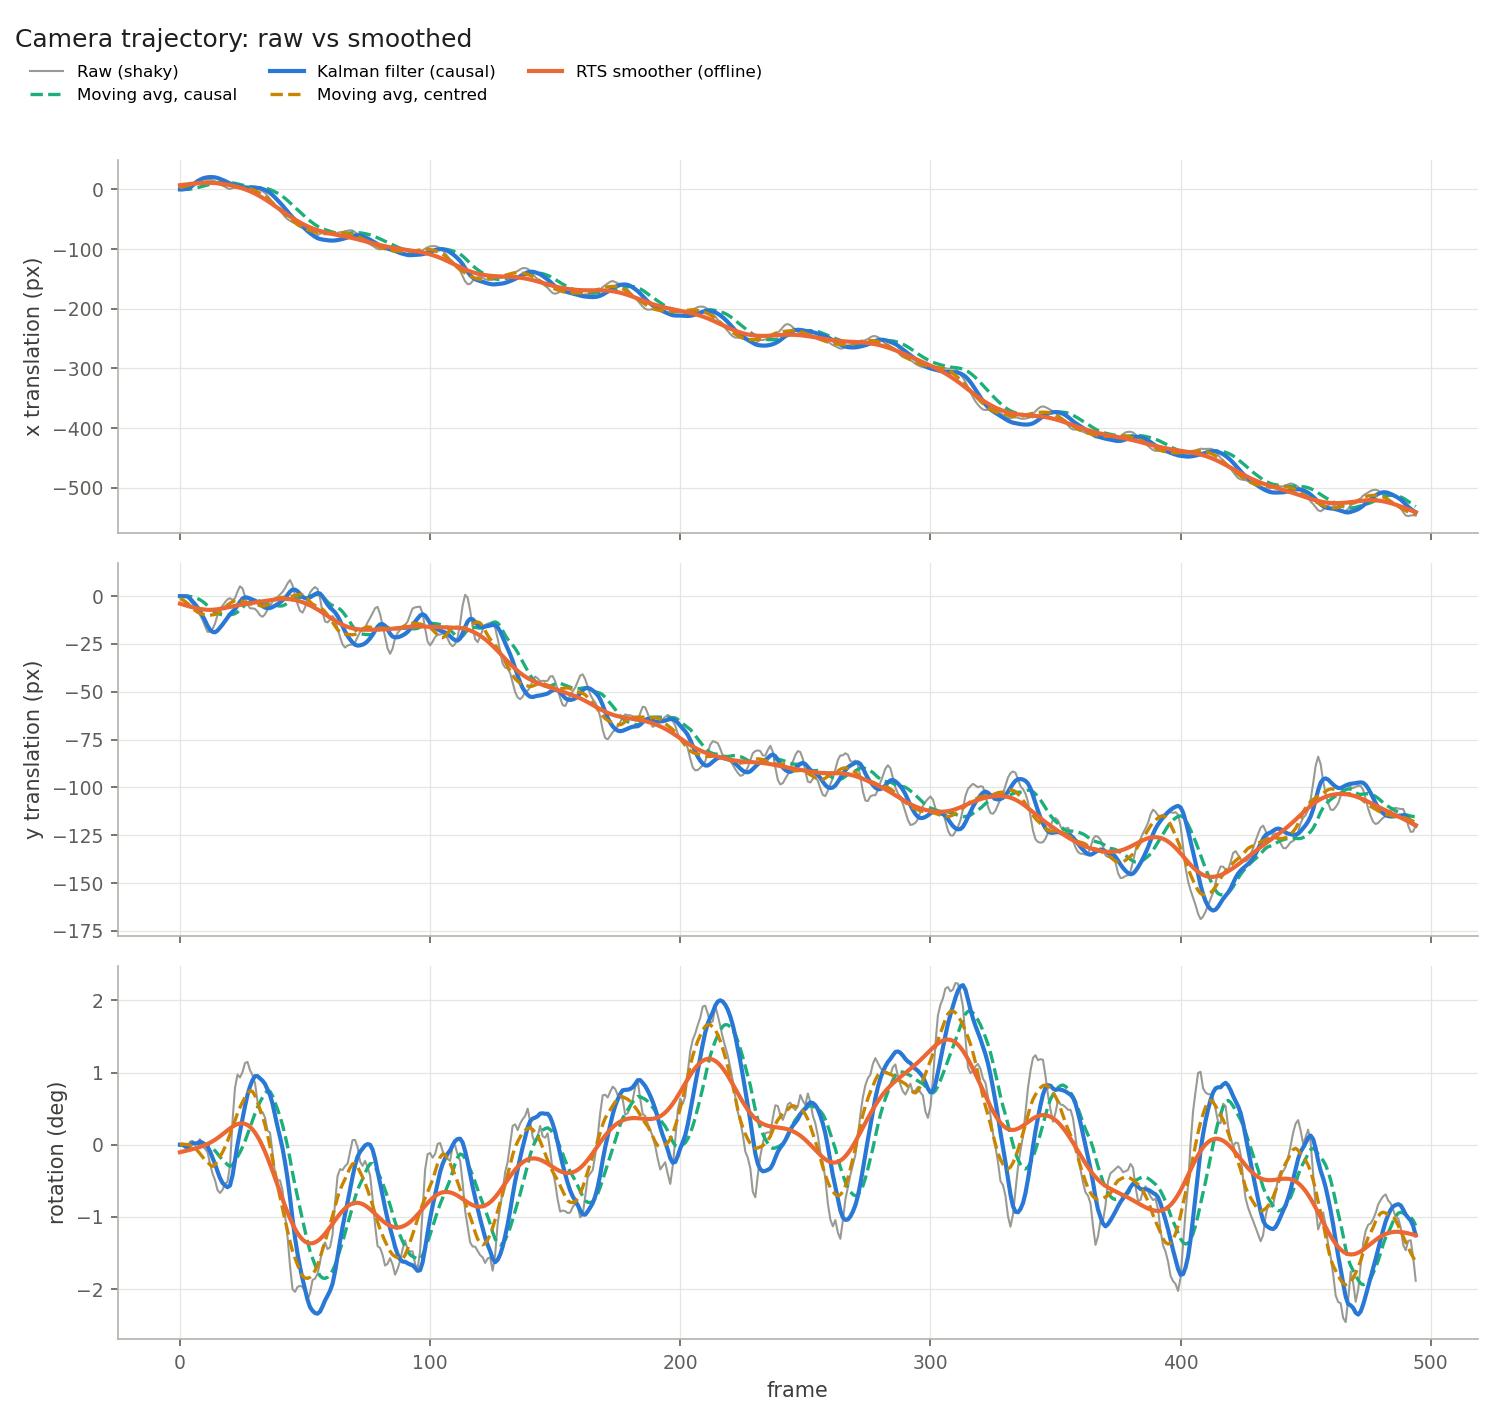
\includegraphics[width=0.85\linewidth]{real_trajectories.png}
  \caption{Camera path on the real video for $x$, $y$ and rotation: the raw (shaky) path and the
  four smoothing methods.}
  \label{fig:real-traj}
\end{figure}

On the trade-off curve (Figure~\ref{fig:real-tradeoff}) the RTS smoother again comes out on top.
This time the Kalman filter lies below the causal moving average: for the same smoothness it
needs less correction (about 30\,px against 42\,px at a jitter of $0.3$). On this video the
model-based filter is therefore the better live choice. Figure~\ref{fig:real-mean} shows the
visual result: over ten frames the raw video is badly blurred, the Kalman filter output is partly
sharp, and the RTS output is sharp except for the car, which really is moving.

\begin{figure}[htbp]
  \centering
  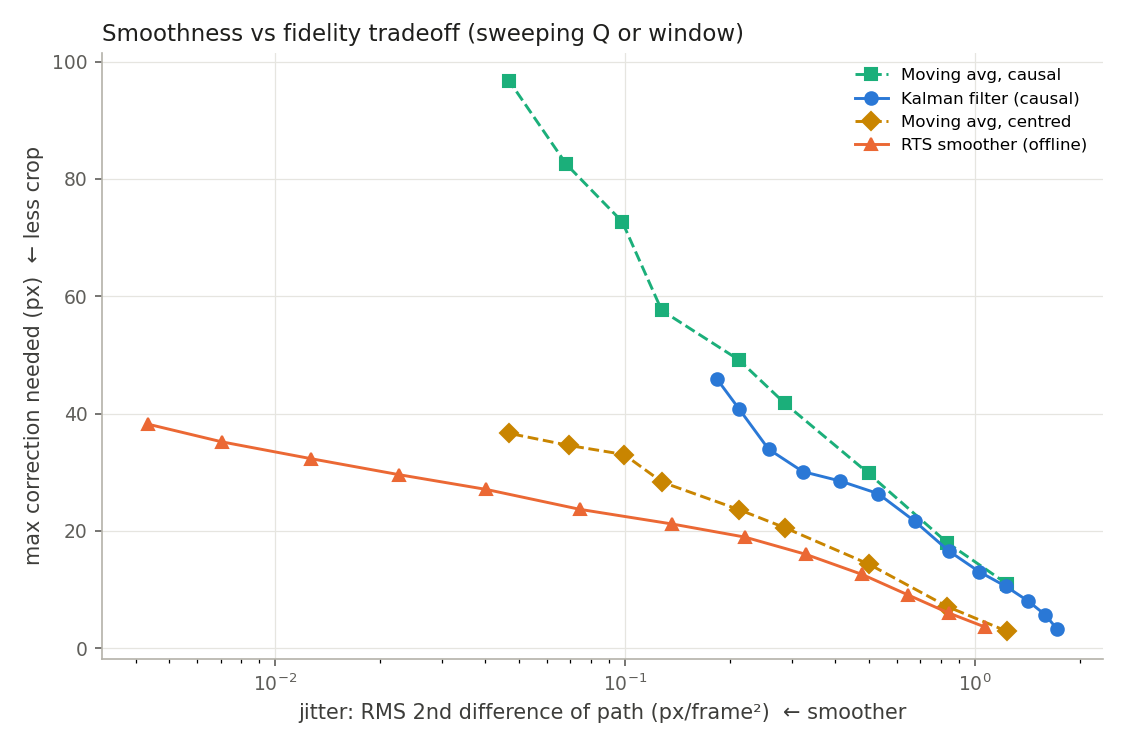
\includegraphics[width=0.7\linewidth]{real_tradeoff_q_sweep.png}
  \caption{Smoothness against required correction on the real video, for a range of settings
  of $\rho$ or the window length. Down and to the left is better.}
  \label{fig:real-tradeoff}
\end{figure}

\begin{figure}[htbp]
  \centering
  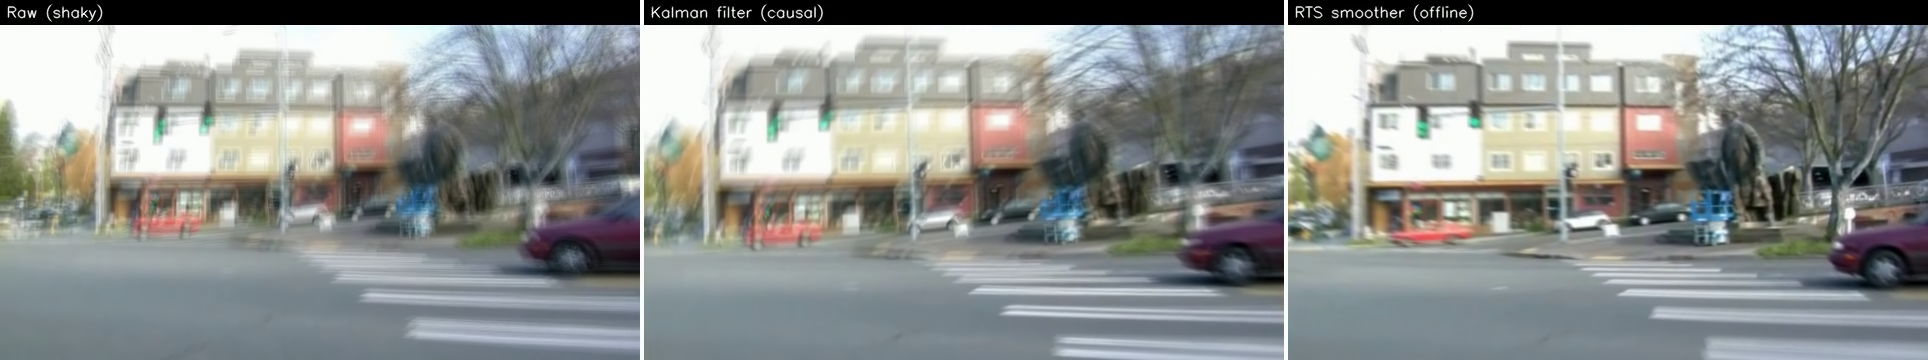
\includegraphics[width=\linewidth]{real_temporal_mean.png}
  \caption{Average of 10 consecutive output frames (frames 60--69) of the real video: raw,
  Kalman filter and RTS smoother. The car in the foreground is moving, so it blurs in every
  panel.}
  \label{fig:real-mean}
\end{figure}

% =====================================================================
\section{Discussion}\label{sec:discussion}
% =====================================================================

\subsection{Is the filter consistent?}\label{sec:consistency}
A Kalman filter predicts not only a value but also how large its error should be ($S_k$). If
its model of the world is right, the actual surprises match that prediction: the NIS averages 1
and about 95\% of innovations fall inside $\pm2\sqrt{S_k}$. Values above that mean the filter is
\emph{over-confident}: it is surprised more often than it expects. Table~\ref{tab:nis} gives the
results, and Figures~\ref{fig:synth-diag} and~\ref{fig:real-diag} show them for the $x$ axis.

\begin{table}[htbp]
  \centering
  \caption{Kalman filter consistency for each axis: mean NIS (ideal 1) and the percentage of
  innovations inside $\pm2\sqrt{S}$ (ideal 95\%).}
  \label{tab:nis}
  \begin{tabular}{lcccc}
    \toprule
    & \multicolumn{2}{c}{Synthetic} & \multicolumn{2}{c}{Real} \\
    \cmidrule(lr){2-3}\cmidrule(lr){4-5}
    Axis & Mean NIS & Inside $\pm2\sqrt{S}$ & Mean NIS & Inside $\pm2\sqrt{S}$ \\
    \midrule
    $x$      & 2.89 & 82\% & 4.83 & 59\% \\
    $y$      & 1.37 & 93\% & 2.00 & 86\% \\
    $\theta$ & 1.14 & 94\% & 4.67 & 58\% \\
    \bottomrule
  \end{tabular}
\end{table}

On the synthetic video, the $y$ and $\theta$ filters are close to consistent. The $x$ filter is
not, and its large surprises are concentrated around the fast pan (Figure~\ref{fig:synth-diag},
frames 130--170): with a small $Q$, the model does not expect a change of speed that large. On the
real video all three axes are over-confident, most of all $x$ and $\theta$.

The main reason shows in the innovation plots: the surprises rise and fall smoothly, instead of
jumping around randomly as they should. Their lag-one autocorrelation (how similar each value is
to the one before) on the $x$ axis is $0.95$ on the synthetic video and $0.97$ on the real one;
a consistent filter would give a value near zero. The model assumes the shake is \emph{white
noise}, independent from one frame to the next, but real hand shake is \emph{coloured}: it
carries on in the same direction for several frames.

Two extensions would deal with the two causes:
\begin{itemize}
  \item add a model of the shake itself to the state (for example a first-order autoregressive
        process), so that shake that persists over several frames is expected;
  \item adapt $Q$ during deliberate pans, or use an interacting multiple-model
        filter~\cite{barshalom2001} that switches to a ``turning'' model when the camera
        manoeuvres.
\end{itemize}

\begin{figure}[htbp]
  \centering
  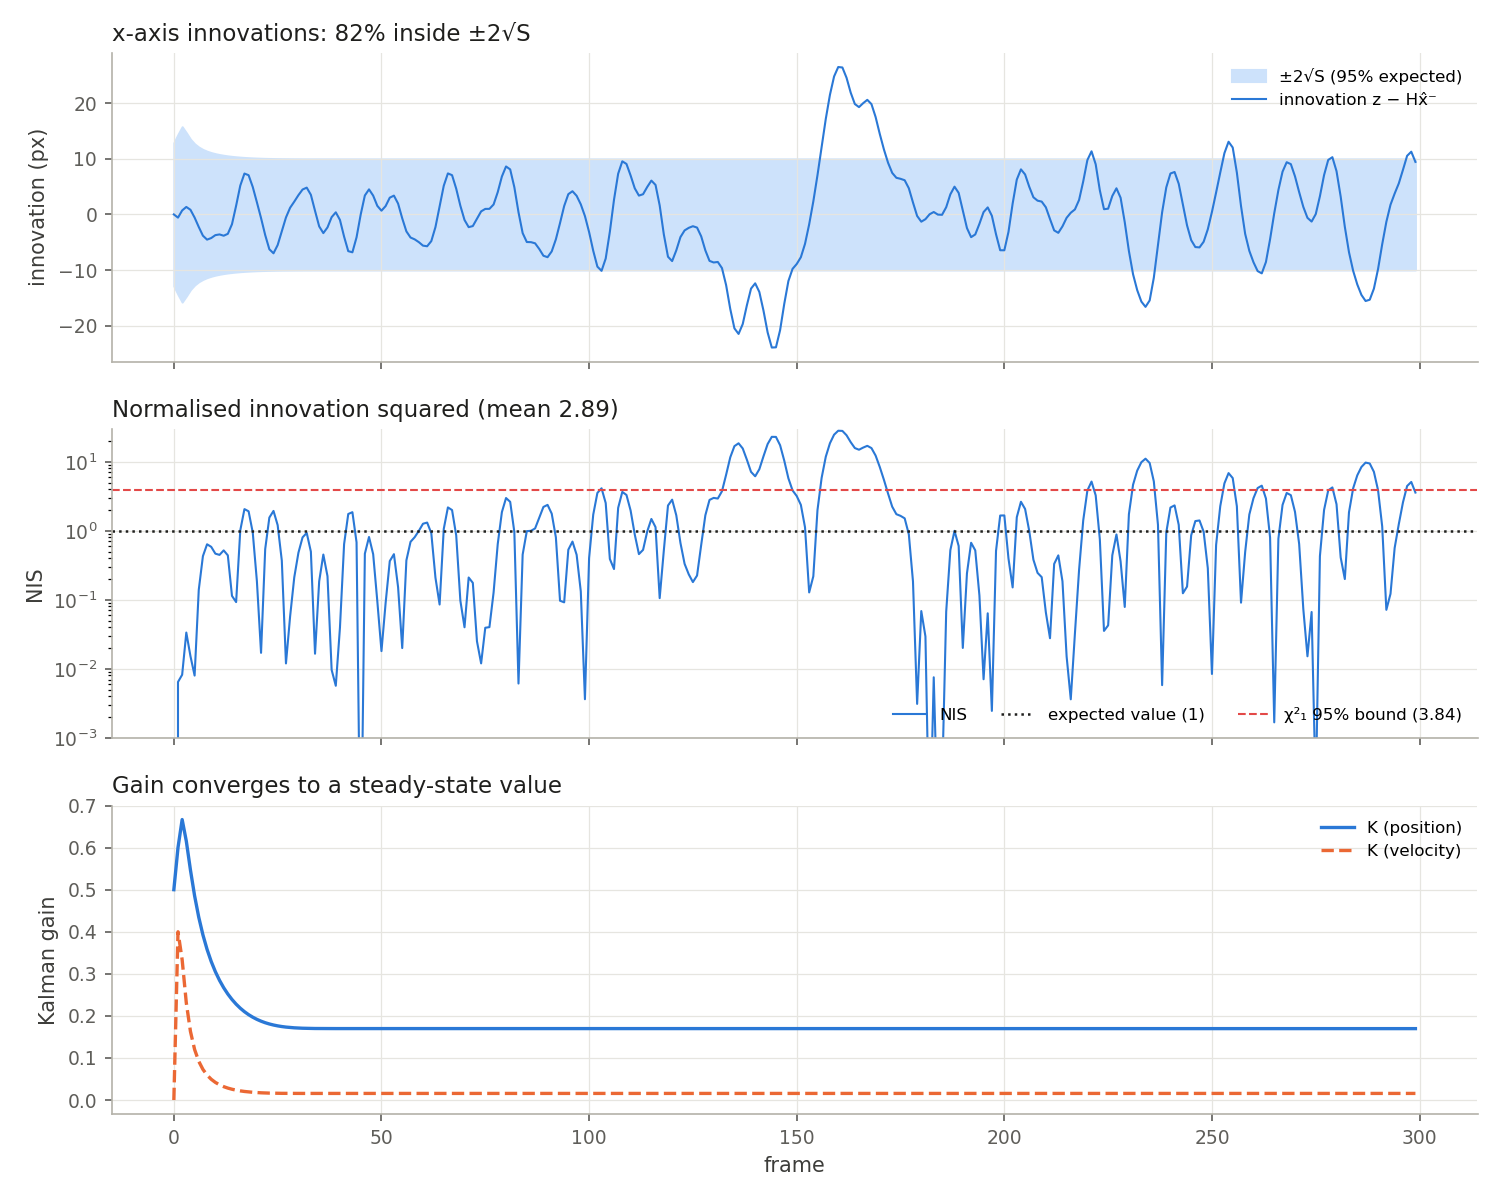
\includegraphics[width=0.72\linewidth]{synth_kf_diagnostics.png}
  \caption{Kalman filter diagnostics on the synthetic video ($x$ axis). Top: innovations with
  the expected $\pm2\sqrt{S}$ band. Middle: NIS with its expected value of 1 and the $\chi^2_1$
  95\% bound. Bottom: the Kalman gain.}
  \label{fig:synth-diag}
\end{figure}

\begin{figure}[htbp]
  \centering
  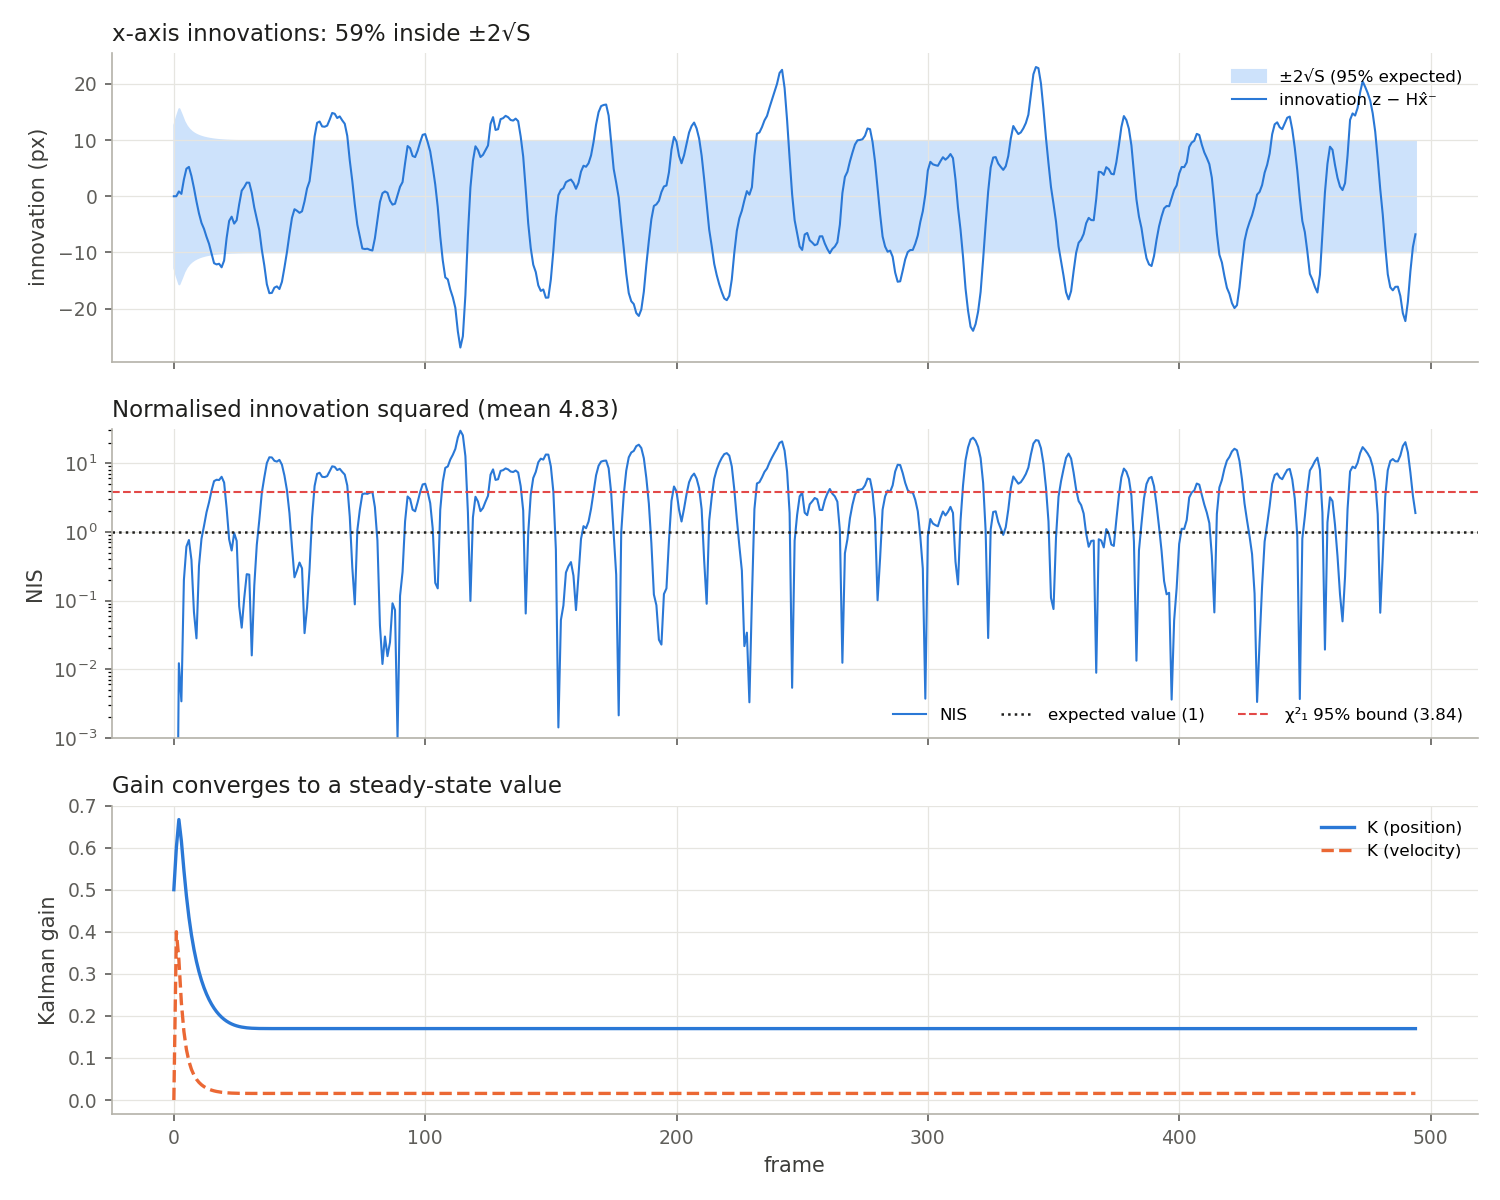
\includegraphics[width=0.72\linewidth]{real_kf_diagnostics.png}
  \caption{Kalman filter diagnostics on the real video ($x$ axis), drawn as in
  Figure~\ref{fig:synth-diag}.}
  \label{fig:real-diag}
\end{figure}

\subsection{What the tuning parameter really does}
The Kalman gain settles within about 30 frames to a fixed value,
$K_\infty = [0.170,\ 0.0158]\T$ (bottom panels of Figures~\ref{fig:synth-diag}
and~\ref{fig:real-diag}). This value depends only on the ratio $\rho = Q/R$, not on $R$ itself,
which is why both videos reach the same value. Once the gain is fixed, the filter becomes a fixed
linear recursion,
$\hat{\mathbf{x}}_k = (I - K_\infty H) F \hat{\mathbf{x}}_{k-1} + K_\infty z_k$, which is a
low-pass filter. Choosing $\rho$ is therefore the same as choosing the filter's cutoff frequency:
how fast a motion has to be before it is treated as shake.

The Kalman formulation still has advantages over a hand-designed low-pass filter. It comes from an
explicit motion model, it reports its own uncertainty (which made the consistency tests above
possible), and it extends naturally to the better models suggested above.

\subsection{Live versus offline}
The gap between the Kalman filter and the RTS smoother is the price of working live. For a
recorded video the RTS smoother is clearly the better choice. The Kalman filter is the right
choice when frames must be stabilised as they arrive, for example in a live stream or on a robot.
It then has to balance smoothness against lag, and as the trade-off curves show, no setting of
$\rho$ gets both.

\subsection{Cropping}
The fixed zoom of 1.12 hides corrections of up to $38.4$\,px horizontally and $21.6$\,px
vertically. On the synthetic video only the causal moving average goes beyond this, in 17 frames
during the pan. On the real video the vertical limit is exceeded by the causal moving average
(19 frames), the Kalman filter (5 frames) and the RTS smoother (4 frames), so brief black borders
can appear. A larger zoom, or one chosen from the corrections actually needed, would remove them
at the cost of a narrower view.

\subsection{Limitations}
\begin{itemize}
  \item The 2D motion model (shift and rotation) cannot represent parallax, changes of
        perspective or rolling-shutter wobble, so strongly three-dimensional scenes keep some
        distortion.
  \item Rotation is measured about the image's corner rather than its centre, which mixes small
        rotations with shifts. This shows up as a slow drift in the synthetic $y$ path towards
        the end of the clip (Figure~\ref{fig:synth-traj}).
  \item Large moving objects can mislead motion estimation if they provide most of the points
        RANSAC keeps.
  \item The estimate of $R$ assumes all shake is faster than a 15-frame moving average can
        follow. Some of the smoothed shake is slower than that, so $R$ is underestimated: on the
        synthetic $x$ axis the estimated shake has a standard deviation of $4.5$\,px, against the
        $6$\,px that was added.
\end{itemize}

% =====================================================================
\section{Conclusion}\label{sec:conclusion}
% =====================================================================
Video stabilisation was treated as estimating a camera's intended path from its measured, shaky
path, using a constant-velocity model with a Kalman filter and an RTS smoother. The main findings
are:
\begin{itemize}
  \item \textbf{Motion estimation is accurate:} the measured path matched the true shaky path to
        within $0.89$\,px.
  \item \textbf{The RTS smoother is the best method for recorded video.} On both videos it gave
        the steadiest and smoothest output, with between a quarter and a third of the jitter of
        the best moving average, and on the synthetic video the lowest error to the true intended
        path.
  \item \textbf{Live stabilisation is a trade-off.} The Kalman filter follows deliberate motion
        with much less lag than a causal moving average but lets more shake through. A single
        ratio, $Q/R$, sets the balance.
  \item \textbf{The model's main weakness is the shake model.} Consistency tests show that the
        filter is over-confident, because real shake persists over several frames instead of
        being independent from frame to frame.
\end{itemize}
The natural next steps are to model the shake as a correlated process and to adapt $Q$ during
deliberate camera turns.

% =====================================================================
\begin{thebibliography}{99}
\bibitem{kalman1960}
R.~E. Kalman, ``A new approach to linear filtering and prediction problems,''
\emph{Journal of Basic Engineering}, vol.~82, no.~1, pp.~35--45, 1960.

\bibitem{rts1965}
H.~E. Rauch, F.~Tung and C.~T. Striebel, ``Maximum likelihood estimates of linear dynamic
systems,'' \emph{AIAA Journal}, vol.~3, no.~8, pp.~1445--1450, 1965.

\bibitem{barshalom2001}
Y.~Bar-Shalom, X.~R. Li and T.~Kirubarajan, \emph{Estimation with Applications to Tracking
and Navigation}. New York: Wiley, 2001.

\bibitem{shitomasi1994}
J.~Shi and C.~Tomasi, ``Good features to track,'' in \emph{Proc.\ IEEE Conf.\ Computer Vision
and Pattern Recognition (CVPR)}, 1994, pp.~593--600.

\bibitem{lucaskanade1981}
B.~D. Lucas and T.~Kanade, ``An iterative image registration technique with an application to
stereo vision,'' in \emph{Proc.\ Int.\ Joint Conf.\ Artificial Intelligence (IJCAI)}, 1981,
pp.~674--679.

\bibitem{bouguet2001}
J.-Y. Bouguet, ``Pyramidal implementation of the affine Lucas Kanade feature tracker:
description of the algorithm,'' Intel Corporation, Technical report, 2001.

\bibitem{fischler1981}
M.~A. Fischler and R.~C. Bolles, ``Random sample consensus: a paradigm for model fitting with
applications to image analysis and automated cartography,'' \emph{Communications of the ACM},
vol.~24, no.~6, pp.~381--395, 1981.

\bibitem{morimoto1998}
C.~Morimoto and R.~Chellappa, ``Evaluation of image stabilization algorithms,'' in
\emph{Proc.\ IEEE Int.\ Conf.\ Acoustics, Speech and Signal Processing (ICASSP)}, 1998,
pp.~2789--2792.

\bibitem{litvin2003}
A.~Litvin, J.~Konrad and W.~C. Karl, ``Probabilistic video stabilization using Kalman filtering
and mosaicking,'' in \emph{Proc.\ SPIE Image and Video Communications and Processing},
vol.~5022, 2003, pp.~663--674.

\bibitem{matsushita2006}
Y.~Matsushita, E.~Ofek, W.~Ge, X.~Tang and H.-Y. Shum, ``Full-frame video stabilization with
motion inpainting,'' \emph{IEEE Trans.\ Pattern Analysis and Machine Intelligence}, vol.~28,
no.~7, pp.~1150--1163, 2006.

\bibitem{grundmann2011}
M.~Grundmann, V.~Kwatra and I.~Essa, ``Auto-directed video stabilization with robust L1 optimal
camera paths,'' in \emph{Proc.\ IEEE Conf.\ Computer Vision and Pattern Recognition (CVPR)},
2011, pp.~225--232.

\bibitem{spoorthiuk}
spoorthiuk (GitHub user), ``Video stabilization using Gaussian and Kalman filters,'' GitHub repository,
\url{https://github.com/spoorthiuk/video-stabilization-using-gaussian-and-kalman-filters}.
\end{thebibliography}

\end{document}
